% Generated by Sphinx.
\def\sphinxdocclass{report}
\documentclass[a4paper,10pt,oneside]{sphinxmanual}

\usepackage[utf8]{inputenc}
\ifdefined\DeclareUnicodeCharacter
  \DeclareUnicodeCharacter{00A0}{\nobreakspace}
\else\fi
\usepackage{cmap}
\usepackage[T1]{fontenc}
\usepackage{amsmath,amssymb}
\usepackage[english]{babel}
\usepackage{times}
\usepackage[Bjarne]{fncychap}
\usepackage{longtable}
\usepackage{sphinx}
\usepackage{multirow}
\usepackage{eqparbox}


\addto\captionsenglish{\renewcommand{\figurename}{Fig. }}
\addto\captionsenglish{\renewcommand{\tablename}{Table }}
\SetupFloatingEnvironment{literal-block}{name=Listing }

\addto\extrasenglish{\def\pageautorefname{page}}

\setcounter{tocdepth}{2}


\title{Devicetree Specification}
\date{24 May 2016}
\release{0.1}
\author{devicetree.org}
\newcommand{\sphinxlogo}{
\includegraphics{devicetree-logo.png}\par}
\renewcommand{\releasename}{Release}
\makeindex

\makeatletter
\def\PYG@reset{\let\PYG@it=\relax \let\PYG@bf=\relax%
    \let\PYG@ul=\relax \let\PYG@tc=\relax%
    \let\PYG@bc=\relax \let\PYG@ff=\relax}
\def\PYG@tok#1{\csname PYG@tok@#1\endcsname}
\def\PYG@toks#1+{\ifx\relax#1\empty\else%
    \PYG@tok{#1}\expandafter\PYG@toks\fi}
\def\PYG@do#1{\PYG@bc{\PYG@tc{\PYG@ul{%
    \PYG@it{\PYG@bf{\PYG@ff{#1}}}}}}}
\def\PYG#1#2{\PYG@reset\PYG@toks#1+\relax+\PYG@do{#2}}

\expandafter\def\csname PYG@tok@gd\endcsname{\def\PYG@tc##1{\textcolor[rgb]{0.63,0.00,0.00}{##1}}}
\expandafter\def\csname PYG@tok@gu\endcsname{\let\PYG@bf=\textbf\def\PYG@tc##1{\textcolor[rgb]{0.50,0.00,0.50}{##1}}}
\expandafter\def\csname PYG@tok@gt\endcsname{\def\PYG@tc##1{\textcolor[rgb]{0.00,0.27,0.87}{##1}}}
\expandafter\def\csname PYG@tok@gs\endcsname{\let\PYG@bf=\textbf}
\expandafter\def\csname PYG@tok@gr\endcsname{\def\PYG@tc##1{\textcolor[rgb]{1.00,0.00,0.00}{##1}}}
\expandafter\def\csname PYG@tok@cm\endcsname{\let\PYG@it=\textit\def\PYG@tc##1{\textcolor[rgb]{0.25,0.50,0.56}{##1}}}
\expandafter\def\csname PYG@tok@vg\endcsname{\def\PYG@tc##1{\textcolor[rgb]{0.73,0.38,0.84}{##1}}}
\expandafter\def\csname PYG@tok@vi\endcsname{\def\PYG@tc##1{\textcolor[rgb]{0.73,0.38,0.84}{##1}}}
\expandafter\def\csname PYG@tok@mh\endcsname{\def\PYG@tc##1{\textcolor[rgb]{0.13,0.50,0.31}{##1}}}
\expandafter\def\csname PYG@tok@cs\endcsname{\def\PYG@tc##1{\textcolor[rgb]{0.25,0.50,0.56}{##1}}\def\PYG@bc##1{\setlength{\fboxsep}{0pt}\colorbox[rgb]{1.00,0.94,0.94}{\strut ##1}}}
\expandafter\def\csname PYG@tok@ge\endcsname{\let\PYG@it=\textit}
\expandafter\def\csname PYG@tok@vc\endcsname{\def\PYG@tc##1{\textcolor[rgb]{0.73,0.38,0.84}{##1}}}
\expandafter\def\csname PYG@tok@il\endcsname{\def\PYG@tc##1{\textcolor[rgb]{0.13,0.50,0.31}{##1}}}
\expandafter\def\csname PYG@tok@go\endcsname{\def\PYG@tc##1{\textcolor[rgb]{0.20,0.20,0.20}{##1}}}
\expandafter\def\csname PYG@tok@cp\endcsname{\def\PYG@tc##1{\textcolor[rgb]{0.00,0.44,0.13}{##1}}}
\expandafter\def\csname PYG@tok@gi\endcsname{\def\PYG@tc##1{\textcolor[rgb]{0.00,0.63,0.00}{##1}}}
\expandafter\def\csname PYG@tok@gh\endcsname{\let\PYG@bf=\textbf\def\PYG@tc##1{\textcolor[rgb]{0.00,0.00,0.50}{##1}}}
\expandafter\def\csname PYG@tok@ni\endcsname{\let\PYG@bf=\textbf\def\PYG@tc##1{\textcolor[rgb]{0.84,0.33,0.22}{##1}}}
\expandafter\def\csname PYG@tok@nl\endcsname{\let\PYG@bf=\textbf\def\PYG@tc##1{\textcolor[rgb]{0.00,0.13,0.44}{##1}}}
\expandafter\def\csname PYG@tok@nn\endcsname{\let\PYG@bf=\textbf\def\PYG@tc##1{\textcolor[rgb]{0.05,0.52,0.71}{##1}}}
\expandafter\def\csname PYG@tok@no\endcsname{\def\PYG@tc##1{\textcolor[rgb]{0.38,0.68,0.84}{##1}}}
\expandafter\def\csname PYG@tok@na\endcsname{\def\PYG@tc##1{\textcolor[rgb]{0.25,0.44,0.63}{##1}}}
\expandafter\def\csname PYG@tok@nb\endcsname{\def\PYG@tc##1{\textcolor[rgb]{0.00,0.44,0.13}{##1}}}
\expandafter\def\csname PYG@tok@nc\endcsname{\let\PYG@bf=\textbf\def\PYG@tc##1{\textcolor[rgb]{0.05,0.52,0.71}{##1}}}
\expandafter\def\csname PYG@tok@nd\endcsname{\let\PYG@bf=\textbf\def\PYG@tc##1{\textcolor[rgb]{0.33,0.33,0.33}{##1}}}
\expandafter\def\csname PYG@tok@ne\endcsname{\def\PYG@tc##1{\textcolor[rgb]{0.00,0.44,0.13}{##1}}}
\expandafter\def\csname PYG@tok@nf\endcsname{\def\PYG@tc##1{\textcolor[rgb]{0.02,0.16,0.49}{##1}}}
\expandafter\def\csname PYG@tok@si\endcsname{\let\PYG@it=\textit\def\PYG@tc##1{\textcolor[rgb]{0.44,0.63,0.82}{##1}}}
\expandafter\def\csname PYG@tok@s2\endcsname{\def\PYG@tc##1{\textcolor[rgb]{0.25,0.44,0.63}{##1}}}
\expandafter\def\csname PYG@tok@nt\endcsname{\let\PYG@bf=\textbf\def\PYG@tc##1{\textcolor[rgb]{0.02,0.16,0.45}{##1}}}
\expandafter\def\csname PYG@tok@nv\endcsname{\def\PYG@tc##1{\textcolor[rgb]{0.73,0.38,0.84}{##1}}}
\expandafter\def\csname PYG@tok@s1\endcsname{\def\PYG@tc##1{\textcolor[rgb]{0.25,0.44,0.63}{##1}}}
\expandafter\def\csname PYG@tok@ch\endcsname{\let\PYG@it=\textit\def\PYG@tc##1{\textcolor[rgb]{0.25,0.50,0.56}{##1}}}
\expandafter\def\csname PYG@tok@m\endcsname{\def\PYG@tc##1{\textcolor[rgb]{0.13,0.50,0.31}{##1}}}
\expandafter\def\csname PYG@tok@gp\endcsname{\let\PYG@bf=\textbf\def\PYG@tc##1{\textcolor[rgb]{0.78,0.36,0.04}{##1}}}
\expandafter\def\csname PYG@tok@sh\endcsname{\def\PYG@tc##1{\textcolor[rgb]{0.25,0.44,0.63}{##1}}}
\expandafter\def\csname PYG@tok@ow\endcsname{\let\PYG@bf=\textbf\def\PYG@tc##1{\textcolor[rgb]{0.00,0.44,0.13}{##1}}}
\expandafter\def\csname PYG@tok@sx\endcsname{\def\PYG@tc##1{\textcolor[rgb]{0.78,0.36,0.04}{##1}}}
\expandafter\def\csname PYG@tok@bp\endcsname{\def\PYG@tc##1{\textcolor[rgb]{0.00,0.44,0.13}{##1}}}
\expandafter\def\csname PYG@tok@c1\endcsname{\let\PYG@it=\textit\def\PYG@tc##1{\textcolor[rgb]{0.25,0.50,0.56}{##1}}}
\expandafter\def\csname PYG@tok@o\endcsname{\def\PYG@tc##1{\textcolor[rgb]{0.40,0.40,0.40}{##1}}}
\expandafter\def\csname PYG@tok@kc\endcsname{\let\PYG@bf=\textbf\def\PYG@tc##1{\textcolor[rgb]{0.00,0.44,0.13}{##1}}}
\expandafter\def\csname PYG@tok@c\endcsname{\let\PYG@it=\textit\def\PYG@tc##1{\textcolor[rgb]{0.25,0.50,0.56}{##1}}}
\expandafter\def\csname PYG@tok@mf\endcsname{\def\PYG@tc##1{\textcolor[rgb]{0.13,0.50,0.31}{##1}}}
\expandafter\def\csname PYG@tok@err\endcsname{\def\PYG@bc##1{\setlength{\fboxsep}{0pt}\fcolorbox[rgb]{1.00,0.00,0.00}{1,1,1}{\strut ##1}}}
\expandafter\def\csname PYG@tok@mb\endcsname{\def\PYG@tc##1{\textcolor[rgb]{0.13,0.50,0.31}{##1}}}
\expandafter\def\csname PYG@tok@ss\endcsname{\def\PYG@tc##1{\textcolor[rgb]{0.32,0.47,0.09}{##1}}}
\expandafter\def\csname PYG@tok@sr\endcsname{\def\PYG@tc##1{\textcolor[rgb]{0.14,0.33,0.53}{##1}}}
\expandafter\def\csname PYG@tok@mo\endcsname{\def\PYG@tc##1{\textcolor[rgb]{0.13,0.50,0.31}{##1}}}
\expandafter\def\csname PYG@tok@kd\endcsname{\let\PYG@bf=\textbf\def\PYG@tc##1{\textcolor[rgb]{0.00,0.44,0.13}{##1}}}
\expandafter\def\csname PYG@tok@mi\endcsname{\def\PYG@tc##1{\textcolor[rgb]{0.13,0.50,0.31}{##1}}}
\expandafter\def\csname PYG@tok@kn\endcsname{\let\PYG@bf=\textbf\def\PYG@tc##1{\textcolor[rgb]{0.00,0.44,0.13}{##1}}}
\expandafter\def\csname PYG@tok@cpf\endcsname{\let\PYG@it=\textit\def\PYG@tc##1{\textcolor[rgb]{0.25,0.50,0.56}{##1}}}
\expandafter\def\csname PYG@tok@kr\endcsname{\let\PYG@bf=\textbf\def\PYG@tc##1{\textcolor[rgb]{0.00,0.44,0.13}{##1}}}
\expandafter\def\csname PYG@tok@s\endcsname{\def\PYG@tc##1{\textcolor[rgb]{0.25,0.44,0.63}{##1}}}
\expandafter\def\csname PYG@tok@kp\endcsname{\def\PYG@tc##1{\textcolor[rgb]{0.00,0.44,0.13}{##1}}}
\expandafter\def\csname PYG@tok@w\endcsname{\def\PYG@tc##1{\textcolor[rgb]{0.73,0.73,0.73}{##1}}}
\expandafter\def\csname PYG@tok@kt\endcsname{\def\PYG@tc##1{\textcolor[rgb]{0.56,0.13,0.00}{##1}}}
\expandafter\def\csname PYG@tok@sc\endcsname{\def\PYG@tc##1{\textcolor[rgb]{0.25,0.44,0.63}{##1}}}
\expandafter\def\csname PYG@tok@sb\endcsname{\def\PYG@tc##1{\textcolor[rgb]{0.25,0.44,0.63}{##1}}}
\expandafter\def\csname PYG@tok@k\endcsname{\let\PYG@bf=\textbf\def\PYG@tc##1{\textcolor[rgb]{0.00,0.44,0.13}{##1}}}
\expandafter\def\csname PYG@tok@se\endcsname{\let\PYG@bf=\textbf\def\PYG@tc##1{\textcolor[rgb]{0.25,0.44,0.63}{##1}}}
\expandafter\def\csname PYG@tok@sd\endcsname{\let\PYG@it=\textit\def\PYG@tc##1{\textcolor[rgb]{0.25,0.44,0.63}{##1}}}

\def\PYGZbs{\char`\\}
\def\PYGZus{\char`\_}
\def\PYGZob{\char`\{}
\def\PYGZcb{\char`\}}
\def\PYGZca{\char`\^}
\def\PYGZam{\char`\&}
\def\PYGZlt{\char`\<}
\def\PYGZgt{\char`\>}
\def\PYGZsh{\char`\#}
\def\PYGZpc{\char`\%}
\def\PYGZdl{\char`\$}
\def\PYGZhy{\char`\-}
\def\PYGZsq{\char`\'}
\def\PYGZdq{\char`\"}
\def\PYGZti{\char`\~}
% for compatibility with earlier versions
\def\PYGZat{@}
\def\PYGZlb{[}
\def\PYGZrb{]}
\makeatother

\renewcommand\PYGZsq{\textquotesingle}

\begin{document}

\maketitle
\tableofcontents
\phantomsection\label{index::doc}


\textbf{Copyright}

\begin{DUlineblock}{0em}
\item[] Copyright 2008,2011 Power.org, Inc.
\item[] Copyright 2008,2011 Freescale Semiconductor, Inc.
\item[] Copyright 2008,2011 International Business Machines Corporation.
\item[] Copyright 2016 Linaro, Ltd.
\item[] Copyright 2016 ARM Ltd.
\end{DUlineblock}

The Linaro and devicetree.org word marks and the Linaro and
devicetree.org logos and related marks are trademarks and service marks
licensed by Linaro Ltd. Implementation of certain elements of this
document may require licenses under third party intellectual property
rights, including without limitation, patent rights. Linaro and its
Members are not, and shall not be held, responsible in any manner for
identifying or failing to identify any or all such third party
intellectual property rights.

The Power Architecture and Power.org word marks and the Power and
Power.org logos and related marks are trademarks and service marks
licensed by Power.org. Implementation of certain elements of this
document may require licenses under third party intellectual property
rights, including without limitation, patent rights. Power.org and its
Members are not, and shall not be held, responsible in any manner for
identifying or failing to identify any or all such third party
intellectual property rights.

THIS SPECIFICATION PROVIDED ``AS IS'' AND WITHOUT ANY WARRANTY
OF ANY KIND, INCLUDING, WITHOUT LIMITATION, ANY EXPRESS OR IMPLIED
WARRANTY OF NON-INFRINGEMENT, MERCHANTABILITY OR FITNESS FOR A
PARTICULAR PURPOSE. IN NO EVENT SHALL LINARO OR ANY MEMBER OF
LINARO BE LIABLE FOR ANY DIRECT, INDIRECT, SPECIAL, EXEMPLARY,
PUNITIVE, OR CONSEQUENTIAL DAMAGES, INCLUDING, WITHOUT LIMITATION, LOST
PROFITS, EVEN IF ADVISED OF THE POSSIBILITY OF SUCH DAMAGES.

Questions pertaining to this document, or the terms or conditions of its
provision, should be addressed to:

\begin{DUlineblock}{0em}
\item[] Linaro, Ltd
\item[] Harston Mill,
\item[] Royston Road,
\item[] Harston CB22 7GG
\item[] Attn: Devicetree.org Board Secretary
\end{DUlineblock}

\textbf{License Information}

Licensed under the Apache License, Version 2.0 (the ``License'');
you may not use this file except in compliance with the License.
You may obtain a copy of the License at

\url{http://www.apache.org/licenses/LICENSE-2.0}

Unless required by applicable law or agreed to in writing, software
distributed under the License is distributed on an ``AS IS'' BASIS,
WITHOUT WARRANTIES OR CONDITIONS OF ANY KIND, either express or implied.
See the License for the specific language governing permissions and
limitations under the License.
\newpage
\textbf{Acknowledgements}

The devicetree.org Technical Steering Committee would like
thank the many individuals and companies that contributed to the
development this specification through writing, technical discussions
and reviews.

We want to thank the power.org Platform Architecture Technical Subcommittee who
developed and published ePAPR. The text of ePAPR was used as the starting
point for this document.

Significant aspects of the Devicetree Specification are based on work done by
the Open Firmware Working Group which developed bindings for IEEE-1275.
We would like to acknowledge their contributions.

We would also like to acknowledge the contribution of the PowerPC and ARM Linux
communities that developed and implemented the flattened devicetree concept.
\phantomsection\label{revhistory:revision-history}

\begin{threeparttable}
\capstart\caption{Revision History}\label{revhistory:id1}
\begin{tabulary}{\linewidth}{| l l J |}
\hline
\textsf{\relax 
Revision
} & \textsf{\relax 
Date
} & \textsf{\relax 
Description
}\\
\hline
DTSpec 0.1
 & 
2016-MAY-24
 & 
Initial prerelease version. Imported ePAPR text
into reStructured Text format and removed Power ISA
specific elements.
\\
\hline\end{tabulary}

\end{threeparttable}



\chapter{Introduction}
\label{introduction:chapter-introduction}\label{introduction:introduction}\label{introduction::doc}\label{introduction:welcome-to-devicetree-specification-s-documentation}

\section{Purpose and Scope}
\label{introduction:purpose-and-scope}
To initialize and boot a computer system, various software components
interact. Firmware might perform low-level initialization of the system
hardware before passing control to software such as an operating system,
bootloader, or hypervisor. Bootloaders and hypervisors can, in turn,
load and transfer control to operating systems. Standard, consistent
interfaces and conventions facilitate the interactions between these
software components.  In this document the term boot program is used to
generically refer to a software component that initializes the system
state and executes another software component referred to as a \emph{client
program}. Examples of a boot programs include: firmware, bootloaders, and
hypervisors. Examples of a client program include: bootloaders,
hypervisors, operating systems, and special purpose programs. A piece of
software may be both a client program and a boot program  (e.g. a hypervisor).

This specification, the Devicetree Specification (DTSpec),
provides a complete boot program to client program
interface definition, combined with minimum system requirements that
facilitate the development of a wide variety of systems.

This specification is targeted towards the requirements of embedded
systems. An embedded system typically consists of system hardware, an
operating system, and application software that are custom designed to
perform a fixed, specific set of tasks. This is unlike general purpose
computers, which are designed to be customized by a user with a variety
of software and I/O devices. Other characteristics of embedded systems
may include:
\begin{itemize}
\item {} 
a fixed set of I/O devices, possibly highly customized for the
application

\item {} 
a system board optimized for size and cost

\item {} 
limited user interface

\item {} 
resource constraints like limited memory and limited nonvolatile storage

\item {} 
real-time constraints

\item {} 
use of a wide variety of operating systems, including Linux,
real-time operating systems, and custom or proprietary operating
systems

\end{itemize}

\textbf{Organization of this Document}
\begin{itemize}
\item {} 
Chapter {\hyperref[introduction:chapter\string-introduction]{\crossref{\DUrole{std,std-ref}{1}}}} introduces the architecture being
specified by DTSpec.

\item {} 
Chapter {\hyperref[devicetree\string-basics:chapter\string-devicetree]{\crossref{\DUrole{std,std-ref}{2}}}} introduces the devicetree concept
and describes its logical structure and standard properties.

\item {} 
Chapter {\hyperref[devicenodes:chapter\string-device\string-node\string-requirements]{\crossref{\DUrole{std,std-ref}{3}}}} specifies the
definition of a base set of device nodes required by DTSpec-compliant
devicetrees.

\item {} 
Chapter {\hyperref[device\string-bindings:chapter\string-device\string-bindings]{\crossref{\DUrole{std,std-ref}{4}}}} describes device bindings for
certain classes of devices and specific device types.

\item {} 
Chapter {\hyperref[flattened\string-format:chapter\string-fdt\string-structure]{\crossref{\DUrole{std,std-ref}{5}}}} specifies the physical structure
of devicetrees.

\end{itemize}

\textbf{Conventions Used in this Document}

The word \emph{shall} is used to indicate mandatory requirements strictly to
be followed in order to conform to the standard and from which no
deviation is permitted (\emph{shall} equals \emph{is required to}).

The word \emph{should} is used to indicate that among several possibilities
one is recommended as particularly suitable, without mentioning or
excluding others; or that a certain course of action is preferred but
not necessarily required; or that (in the negative form) a certain
course of action is deprecated but not prohibited (\emph{should} equals \emph{is
recommended that}).

The word \emph{may} is used to indicate a course of action permissible within
the limits of the standard (\emph{may} equals \emph{is permitted}).

Examples of devicetree constructs are frequently shown in \emph{Devicetree
Syntax} form. See section {\hyperref[source\string-language:chapter\string-devicetree\string-source\string-format]{\crossref{\DUrole{std,std-ref}{6}}}} for
an overview of this syntax.


\section{Relationship to IEEE™ 1275 and ePAPR}
\label{introduction:relationship-to-ieee-1275-and-epapr}
DTSpec is loosely related to the IEEE 1275 Open Firmware
standard—\emph{IEEE Standard for Boot (Initialization Configuration)
Firmware: Core Requirements and Practices} \phantomsection\label{introduction:id1}{\hyperref[references:ieee1275]{\crossref{{[}IEEE1275{]}}}}.

The original IEEE 1275 specification and its derivatives such as CHRP \phantomsection\label{introduction:id2}{\hyperref[references:chrp]{\crossref{{[}CHRP{]}}}}
and PAPR \phantomsection\label{introduction:id3}{\hyperref[references:papr]{\crossref{{[}PAPR{]}}}} address problems of general purpose computers, such as how a
single version of an operating system can work on several different
computers within the same family and the problem of loading an operating
system from user-installed I/O devices.

Because of the nature of embedded systems, some of these problems faced
by open, general purpose computers do not apply. Notable features of the
IEEE 1275 specification that are omitted from the DTSpec include:
\begin{itemize}
\item {} 
Plug-in device drivers

\item {} 
FCode

\item {} 
The programmable Open Firmware user interface based on Forth

\item {} 
FCode debugging

\item {} 
Operating system debugging

\end{itemize}

What is retained from IEEE-1275 are concepts from the devicetree
architecture by which a boot program can describe and communicate system
hardware information to client program, thus eliminating the need for
the client program to have hard-coded descriptions of system hardware.

This specification partially supersedes the ePAPR {[}EPAPR{]} specification.
ePAPR documents how devicetree is used by the PowerISA, and covers both
general concepts, as well as PowerISA specific bindings.
The text of this document was derived from ePAPR, but either removes architecture specific bindings, or moves them into an appendix.


\section{32-bit and 64-bit Support}
\label{introduction:bit-and-64-bit-support}
The DTSpec supports CPUs with both 32-bit and 64-bit addressing
capabilities. Where applicable, sections of the DTSpec describe any
requirements or considerations for 32-bit and 64-bit addressing.


\section{Definition of Terms}
\label{introduction:definition-of-terms}\begin{description}
\item[{AMP\index{AMP|textbf}}] \leavevmode\phantomsection\label{introduction:term-amp}
Asymmetric Multiprocessing. Computer available CPUs are partitioned into
groups, each running a distinct operating system image. The CPUs
may or not may not be identical.

\item[{boot CPU\index{boot CPU|textbf}}] \leavevmode\phantomsection\label{introduction:term-boot-cpu}
The first CPU which a boot program directs to a client program’s
entry point.

\item[{Book III-E\index{Book III-E|textbf}}] \leavevmode\phantomsection\label{introduction:term-book-iii-e}
Embedded Environment. Section of the Power ISA defining supervisor
instructions and related facilities used in embedded Power processor
implementations.

\item[{boot program\index{boot program|textbf}}] \leavevmode\phantomsection\label{introduction:term-boot-program}
Used to generically refer to a software component that initializes
the system state and executes another software component referred to
as a client program. Examples of a boot programs include: firmware,
bootloaders, and hypervisors.

\item[{client program\index{client program|textbf}}] \leavevmode\phantomsection\label{introduction:term-client-program}
Program that typically contains application or operating system
software. Examples of a client program include: bootloaders,
hypervisors, operating systems, and special purpose programs.

\item[{cell\index{cell|textbf}}] \leavevmode\phantomsection\label{introduction:term-cell}
A unit of information consisting of 32 bits.

\item[{DMA\index{DMA|textbf}}] \leavevmode\phantomsection\label{introduction:term-dma}
Direct memory access

\item[{DTB\index{DTB|textbf}}] \leavevmode\phantomsection\label{introduction:term-dtb}
Devicetree blob. Compact binary representation of the devicetree.

\item[{DTC\index{DTC|textbf}}] \leavevmode\phantomsection\label{introduction:term-dtc}
Devicetree compiler. An open source tool used to create DTB files
from DTS files.

\item[{DTS\index{DTS|textbf}}] \leavevmode\phantomsection\label{introduction:term-dts}
Devicetree syntax. A textual representation of a devicetree
consumed by the DTC. See Appendix A Devicetree Source Format
(version 1).

\item[{effective address\index{effective address|textbf}}] \leavevmode\phantomsection\label{introduction:term-effective-address}
Memory address as computed by processor storage access or branch
instruction.

\item[{physical address\index{physical address|textbf}}] \leavevmode\phantomsection\label{introduction:term-physical-address}
Address used by the processor to access external device, typically a
memory controller.

\item[{Power ISA\index{Power ISA|textbf}}] \leavevmode\phantomsection\label{introduction:term-power-isa}
Power Instruction Set Architecture.

\item[{interrupt specifier\index{interrupt specifier|textbf}}] \leavevmode\phantomsection\label{introduction:term-interrupt-specifier}
A property value that describes an interrupt. Typically information
that specifies an interrupt number and sensitivity and triggering
mechanism is included.

\item[{secondary CPU\index{secondary CPU|textbf}}] \leavevmode\phantomsection\label{introduction:term-secondary-cpu}
CPUs other than the boot CPU that belong to the client program are
considered \emph{secondary CPUs}.

\item[{SMP\index{SMP|textbf}}] \leavevmode\phantomsection\label{introduction:term-smp}
Symmetric multiprocessing. A computer architecture where two or more
identical CPUs can share memory and IO and operate under a single operating
system.

\item[{SoC\index{SoC|textbf}}] \leavevmode\phantomsection\label{introduction:term-soc}
System on a chip. A single computer chip integrating one or more CPU
core as well as number of other peripherals.

\item[{unit address\index{unit address|textbf}}] \leavevmode\phantomsection\label{introduction:term-unit-address}
The part of a node name specifying the node’s address in the address
space of the parent node.

\item[{quiescent CPU\index{quiescent CPU|textbf}}] \leavevmode\phantomsection\label{introduction:term-quiescent-cpu}
A quiescent CPU is in a state where it cannot interfere with the
normal operation of other CPUs, nor can its state be affected by the
normal operation of other running CPUs, except by an explicit method
for enabling or re-enabling the quiescent CPU.

\end{description}


\chapter{The Devicetree}
\label{devicetree-basics:chapter-devicetree}\label{devicetree-basics:the-devicetree}\label{devicetree-basics::doc}

\section{Overview}
\label{devicetree-basics:overview}
DTSpec specifies a construct called a \emph{devicetree} to describe
system hardware. A boot program loads a devicetree into a client
program’s memory and passes a pointer to the devicetree to the client.

This chapter describes the logical structure of the devicetree and
specifies a base set of properties for use in describing device nodes.
Chapter {\hyperref[devicenodes:chapter\string-device\string-node\string-requirements]{\crossref{\DUrole{std,std-ref}{3}}}} specifies certain device nodes
required by a DTSpec compliant
devicetree. Chapter 6 describes the DTSpec defined device bindings— the
requirements for representing certain device types classes of devices.
Chapter 8 describes the in-memory encoding of the devicetree.

A devicetree is a tree data structure with nodes that describe the
devices in a system. Each node has property/value pairs that describe
the characteristics of the device being represented. Each node has
exactly one parent except for the root node, which has no parent.

An DTSpec-compliant devicetree describes device information in a system
that cannot necessarily be dynamically detected by a client program. For
example, the architecture of PCI enables a client to probe and detect
attached devices, and thus devicetree nodes describing PCI devices
might not be required. However, a device node is required to describe a
PCI host bridge device in the system if it cannot be detected by
probing.

\textbf{Example}

\hyperref[devicetree-basics:example-simple-devicetree]{Fig. \ref{devicetree-basics:example-simple-devicetree}} shows an example representation of a
simple devicetree that is nearly
complete enough to boot a simple operating system, with the platform
type, CPU, and memory described. Device nodes are shown with properties
and values shown beside the node.
\begin{figure}[htbp]
\centering
\capstart

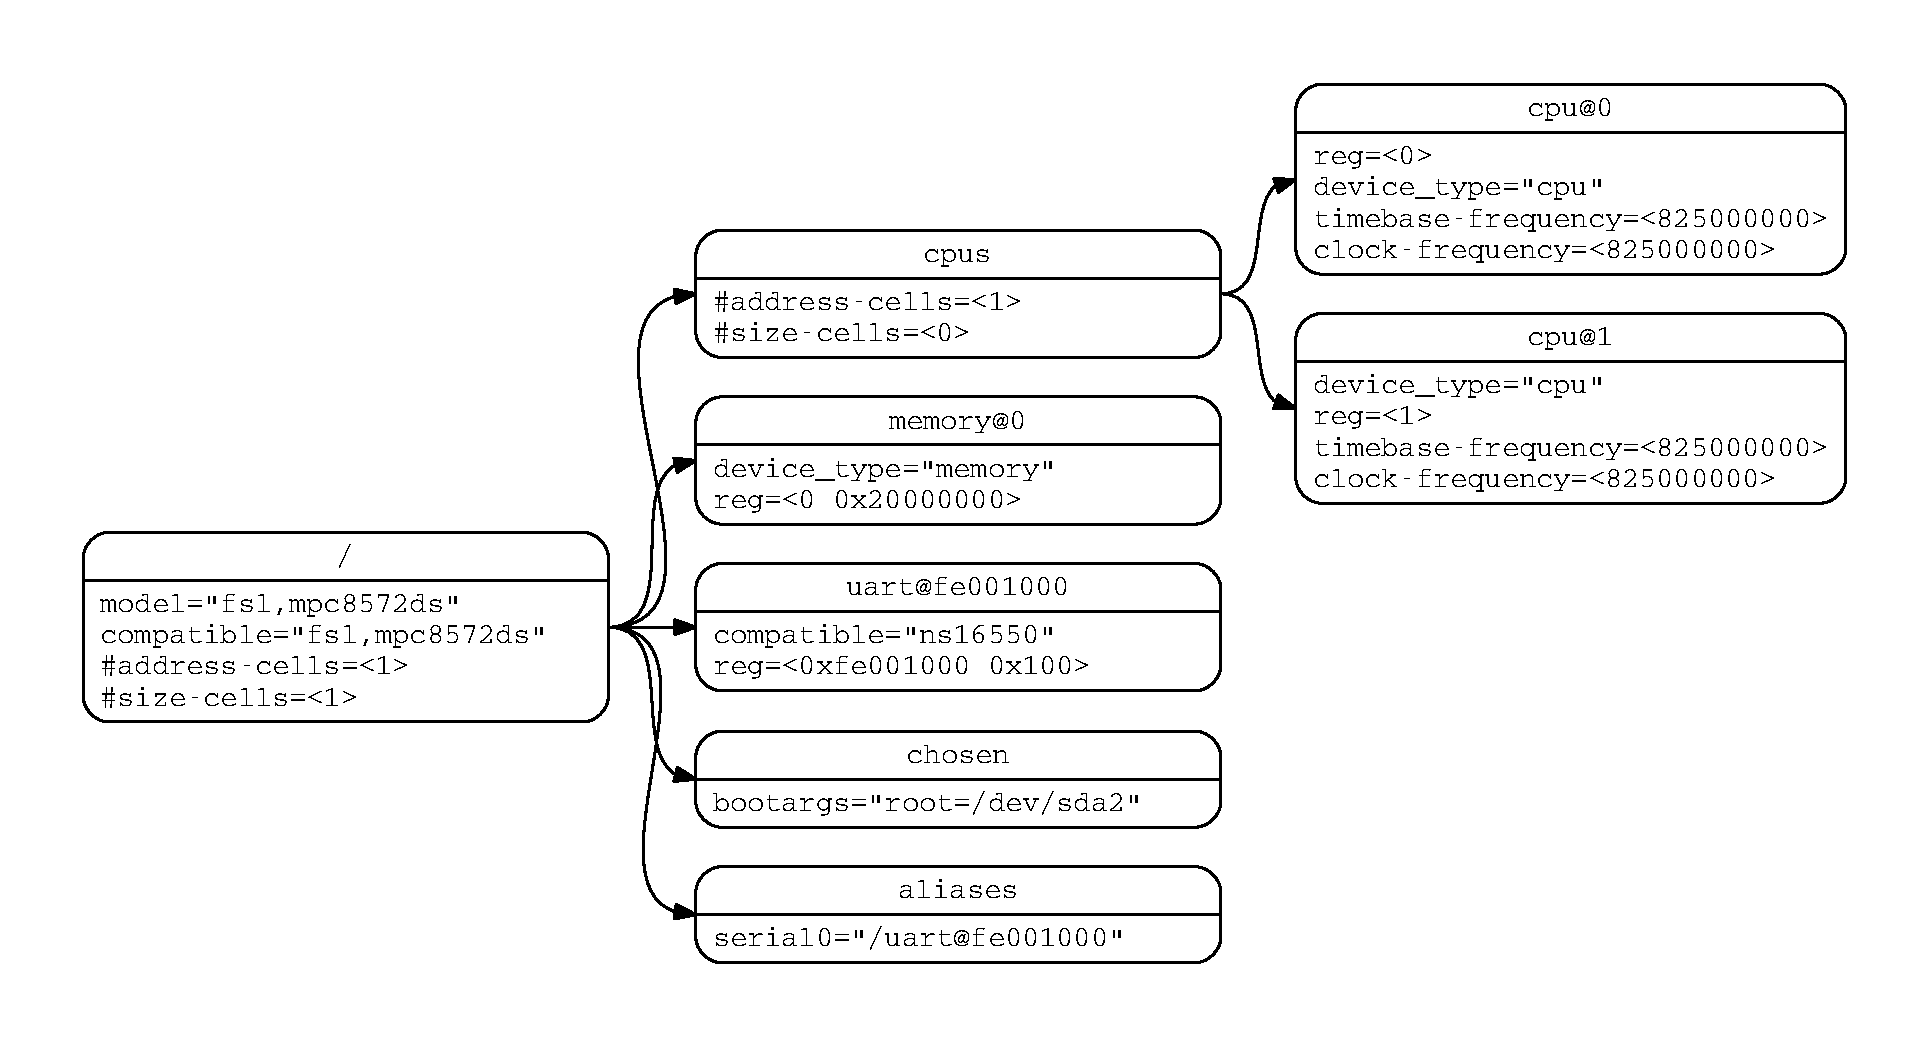
\includegraphics{graphviz-e69f9031183bd8d3b6636722c922fcb66d4843c4.pdf}
\caption{Devicetree Example}\label{devicetree-basics:example-simple-devicetree}\label{devicetree-basics:id3}\end{figure}


\section{Devicetree Structure and Conventions}
\label{devicetree-basics:devicetree-structure-and-conventions}

\subsection{Node Names}
\label{devicetree-basics:node-names}\label{devicetree-basics:sect-node-names}

\subsubsection{Node Name Requirements}
\label{devicetree-basics:node-name-requirements}
Each node in the devicetree is named according to the following
convention:
\begin{quote}

\code{node-name@unit-address}
\end{quote}

The \emph{node-name} component specifies the name of the node. It shall be 1
to 31 characters in length and consist solely of characters from the set
of characters in \hyperref[devicetree-basics:node-name-characters]{Table \ref{devicetree-basics:node-name-characters}}.


\begin{threeparttable}
\capstart\caption{Valid characters for node names}\label{devicetree-basics:node-name-characters}\label{devicetree-basics:id4}
\begin{tabulary}{\linewidth}{| c p{8cm} |}
\hline
\textsf{\relax 
Character
} & \textsf{\relax 
Description
}\\
\hline
\code{0-9}
 & 
digit
\\
\hline
\code{a-z}
 & 
lowercase letter
\\
\hline
\code{A-Z}
 & 
uppercase letter
\\
\hline
\code{,}
 & 
comma
\\
\hline
\code{.}
 & 
period
\\
\hline
\code{\_}
 & 
underscore
\\
\hline
\code{+}
 & 
plus sign
\\
\hline
\code{-}
 & 
dash
\\
\hline\end{tabulary}

\end{threeparttable}


The \emph{node-name} shall start with a lower or uppercase character and
should describe the general class of device.

The \emph{unit-address} component of the name is specific to the bus type on
which the node sits. It consists of one or more ASCII characters from
the set of characters in \hyperref[devicetree-basics:node-name-characters]{Table \ref{devicetree-basics:node-name-characters}}. The
unit-address must match the first
address specified in the \emph{reg} property of the node. If the node has no
\emph{reg} property, the \emph{@unit-address} must be omitted and the
\emph{node-name} alone differentiates the node from other nodes at the same
level in the tree. The binding for a particular bus may specify
additional, more specific requirements for the format of \emph{reg} and the
\emph{unit-address}.

The root node does not have a node-name or unit-address. It is
identified by a forward slash (/).
\begin{figure}[htbp]
\centering
\capstart

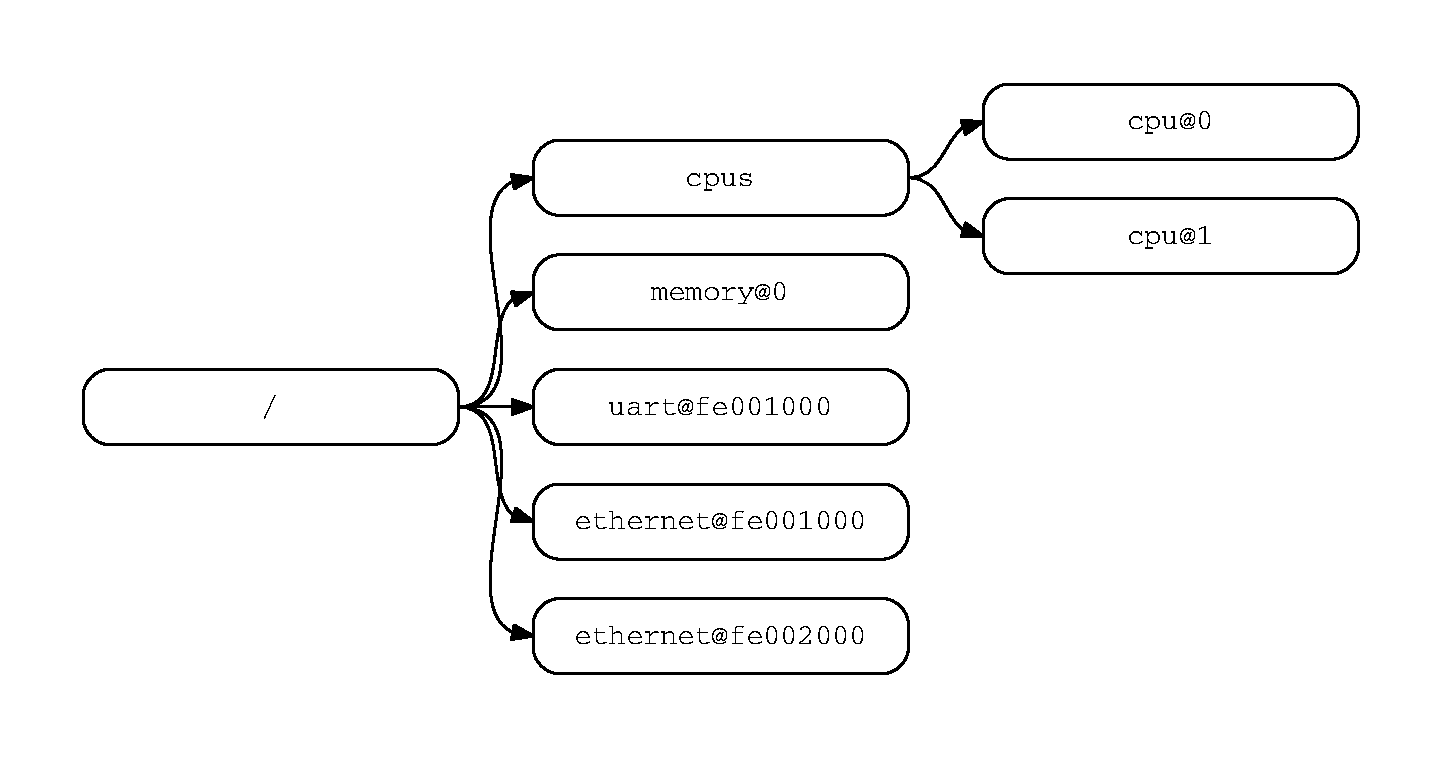
\includegraphics{graphviz-8bc6c34d442f7e613c5d327992e204083ddaf50f.pdf}
\caption{Examples of Node Names}\label{devicetree-basics:example-nodenames}\label{devicetree-basics:id5}\end{figure}

In \hyperref[devicetree-basics:example-nodenames]{Fig. \ref{devicetree-basics:example-nodenames}}:
\begin{itemize}
\item {} 
The nodes with the name cpu are distinguished by their unit-address
values of 0 and 1.

\item {} 
The nodes with the name Ethernet are distinguished by their
unit-address values of FE001000 and FE002000.

\end{itemize}


\subsection{Generic Names Recommendation}
\label{devicetree-basics:generic-names-recommendation}
The name of a node should be somewhat generic, reflecting the function
of the device and not its precise programming model. If appropriate, the
name should be one of the following choices:
\begin{itemize}\setlength{\itemsep}{0pt}\setlength{\parskip}{0pt}
\item {} 
atm

\item {} 
cache-controller

\item {} 
compact-flash

\item {} 
can

\item {} 
cpu

\item {} 
crypto

\item {} 
disk

\item {} 
display

\item {} 
dma-controller

\item {} 
ethernet

\item {} 
ethernet-phy

\item {} 
fdc

\item {} 
flash

\item {} 
gpio

\item {} 
i2c

\item {} 
ide

\item {} 
interrupt-controller

\item {} 
isa

\item {} 
keyboard

\item {} 
mdio

\item {} 
memory

\item {} 
memory-controller

\item {} 
mouse

\item {} 
nvram

\item {} 
parallel

\item {} 
pc-card

\item {} 
pci

\item {} 
pcie

\item {} 
rtc

\item {} 
sata

\item {} 
scsi

\item {} 
serial

\item {} 
sound

\item {} 
spi

\item {} 
timer

\item {} 
usb

\item {} 
vme

\item {} 
watchdog

\end{itemize}


\subsection{Path Names}
\label{devicetree-basics:path-names}
A node in the devicetree can be uniquely identified by specifying the
full path from the root node, through all descendant nodes, to the
desired node.

The convention for specifying a device path is:
\begin{quote}

\code{/node-name-1/node-name-2/node-name-N}
\end{quote}

For example, in \hyperref[devicetree-basics:example-nodenames]{Fig. \ref{devicetree-basics:example-nodenames}}, the device path to cpu \#1 would be:
\begin{quote}

\code{/cpus/cpu@1}
\end{quote}

The path to the root node is /.

A unit address may be omitted if the full path to the node is
unambiguous.

If a client program encounters an ambiguous path, its behavior is
undefined.


\subsection{Properties}
\label{devicetree-basics:properties}
Each node in the devicetree has properties that describe the
characteristics of the node. Properties consist of a name and a value.


\subsubsection{Property Names}
\label{devicetree-basics:property-names}
Property names are strings of 1 to 31 characters from the characters show in
\hyperref[devicetree-basics:property-name-characters]{Table \ref{devicetree-basics:property-name-characters}}


\begin{threeparttable}
\capstart\caption{Valid characters for property names}\label{devicetree-basics:property-name-characters}\label{devicetree-basics:id6}
\begin{tabulary}{\linewidth}{| c p{8cm} |}
\hline
\textsf{\relax 
Character
} & \textsf{\relax 
Description
}\\
\hline
\code{0-9}
 & 
digit
\\
\hline
\code{a-z}
 & 
lowercase letter
\\
\hline
\code{A-Z}
 & 
uppercase letter
\\
\hline
\code{,}
 & 
comma
\\
\hline
\code{.}
 & 
period
\\
\hline
\code{\_}
 & 
underscore
\\
\hline
\code{+}
 & 
plus sign
\\
\hline
\code{?}
 & 
question mark
\\
\hline
\code{\#}
 & 
hash
\\
\hline\end{tabulary}

\end{threeparttable}


Nonstandard property names should specify a unique string prefix, such
as a stock ticker symbol, identifying the name of the company or
organization that defined the property. Examples:
\begin{quote}

\begin{DUlineblock}{0em}
\item[] \code{fsl,channel-fifo-len}
\item[] \code{ibm,ppc-interrupt-server\#s}
\item[] \code{linux,network-index}
\end{DUlineblock}
\end{quote}


\subsubsection{Property Values}
\label{devicetree-basics:sect-property-values}\label{devicetree-basics:property-values}
A property value is an array of zero or more bytes that contain
information associated with the property.

Properties might have an empty value if conveying true-false
information. In this case, the presence or absence of the property is
sufficiently descriptive.

\hyperref[devicetree-basics:property-values-table]{Table \ref{devicetree-basics:property-values-table}} describes the set of basic value types defined by the DTSpec.

\begin{longtable}{| p{4cm} p{12cm} |}
\caption{Property values}\label{devicetree-basics:property-values-table}\\
\hline
\textsf{\relax 
Value
} & \textsf{\relax 
Description
}\\
\hline\endfirsthead

\multicolumn{2}{c}%
{{\tablecontinued{\tablename\ \thetable{} -- continued from previous page}}} \\
\hline
\textsf{\relax 
Value
} & \textsf{\relax 
Description
}\\
\hline\endhead

\hline \multicolumn{2}{|r|}{{\tablecontinued{Continued on next page}}} \\ \hline
\endfoot

\endlastfoot


\code{\textless{}empty\textgreater{}}
 & 
Value is empty. Used for conveying true-false information, when
the presence or absence of the property itself is sufficiently
descriptive.
\\
\hline
\code{\textless{}u32\textgreater{}}
 & 
A 32-bit integer in big-endian format. Example: the 32-bit value
0x11223344 would be represented in memory as:
\begin{quote}

\begin{OriginalVerbatim}[commandchars=\\\{\}]
address    11
address+1  22
address+2  33
address+3  44
\end{OriginalVerbatim}
\end{quote}
\\
\hline
\code{\textless{}u64\textgreater{}}
 & 
Represents a 64-bit integer in big-endian format. Consists of
two \code{\textless{}u32\textgreater{}} values where the first value contains the most
significant bits of the integer and the second value contains
the least significant bits.

Example: the 64-bit value 0x1122334455667788 would be
represented as two cells as: \code{\textless{}0x11223344 0x55667788\textgreater{}}.

The value would be represented in memory as:
\begin{quote}

\begin{OriginalVerbatim}[commandchars=\\\{\}]
  address  11
address+1  22
address+2  33
address+3  44
address+4  55
address+5  66
address+6  77
address+7  88
\end{OriginalVerbatim}
\end{quote}
\\
\hline
\code{\textless{}string\textgreater{}}
 & 
Strings are printable and null-terminated. Example: the string
``hello'' would be represented in memory as:
\begin{quote}

\begin{OriginalVerbatim}[commandchars=\\\{\}]
  address  68  \PYGZsq{}h\PYGZsq{}
address+1  65  \PYGZsq{}e\PYGZsq{}
address+2  6C  \PYGZsq{}l\PYGZsq{}
address+3  6C  \PYGZsq{}l\PYGZsq{}
address+4  6F  \PYGZsq{}o\PYGZsq{}
address+5  00  \PYGZsq{}\PYGZbs{}0\PYGZsq{}
\end{OriginalVerbatim}
\end{quote}
\\
\hline
\code{\textless{}prop-encoded-array\textgreater{}}
 & 
Format is specific to the property. See the property definition.
\\
\hline
\code{\textless{}phandle\textgreater{}}
 & 
A \code{\textless{}u32\textgreater{}} value. A \emph{phandle} value is a way to reference another
node in the devicetree. Any node that can be referenced defines
a phandle property with a unique \code{\textless{}u32\textgreater{}} value. That number
is used for the value of properties with a phandle value
type.
\\
\hline
\code{\textless{}stringlist\textgreater{}}
 & 
A list of \code{\textless{}string\textgreater{}} values concatenated together.

Example: The string list ``hello'',''world'' would be represented in
memory as:
\begin{quote}

\begin{OriginalVerbatim}[commandchars=\\\{\}]
   address  68  \PYGZsq{}h\PYGZsq{}
 address+1  65  \PYGZsq{}e\PYGZsq{}
 address+2  6C  \PYGZsq{}l\PYGZsq{}
 address+3  6C  \PYGZsq{}l\PYGZsq{}
 address+4  6F  \PYGZsq{}o\PYGZsq{}
 address+5  00  \PYGZsq{}\PYGZbs{}0\PYGZsq{}
 address+6  77  \PYGZsq{}w\PYGZsq{}
 address+7  6f  \PYGZsq{}o\PYGZsq{}
 address+8  72  \PYGZsq{}r\PYGZsq{}
 address+9  6C  \PYGZsq{}l\PYGZsq{}
address+10  64  \PYGZsq{}d\PYGZsq{}
address+11  00  \PYGZsq{}\PYGZbs{}0\PYGZsq{}
\end{OriginalVerbatim}
\end{quote}
\\
\hline\end{longtable}



\section{Standard Properties}
\label{devicetree-basics:standard-properties}\label{devicetree-basics:sect-standard-properties}
DTSpec specifies a set of standard properties for device nodes. These
properties are described in detail in this section. Device nodes defined
by DTSpec (see Chapter {\hyperref[devicenodes:chapter\string-device\string-node\string-requirements]{\crossref{\DUrole{std,std-ref}{3}}}}) may specify
additional requirements or constraints regarding the use of the standard
properties. Chapter {\hyperref[device\string-bindings:chapter\string-device\string-bindings]{\crossref{\DUrole{std,std-ref}{4}}}} describes the representation
of specific devices may also specify additional requirements.

\begin{notice}{note}{Note:}
All examples of devicetree nodes in this document use the
\textsc{DTS} (Devicetree Source) format for specifying nodes and properties.
\end{notice}


\subsection{compatible}
\label{devicetree-basics:compatible}\label{devicetree-basics:sect-standard-properties-compatible}
Property name: \code{compatible}

Value type: \code{\textless{}stringlist\textgreater{}}

Description:
\begin{quote}

The \emph{compatible} property value consists of one or more strings that
define the specific programming model for the device. This list of
strings should be used by a client program for device driver selection.
The property value consists of a concatenated list of null terminated
strings, from most specific to most general. They allow a device to
express its compatibility with a family of similar devices, potentially
allowing a single device driver to match against several devices.

The recommended format is \code{"manufacturer,model"}, where
\code{manufacturer} is a string describing the name of the manufacturer
(such as a stock ticker symbol), and \code{model} specifies the model
number.
\end{quote}

Example:
\begin{quote}

\code{compatible = "fsl,mpc8641-uart", "ns16550";}

In this example, an operating system would first try to locate a device
driver that supported fsl,mpc8641-uart. If a driver was not found, it
would then try to locate a driver that supported the more general
ns16550 device type.
\end{quote}


\subsection{model}
\label{devicetree-basics:model}
Property name: \code{model}

Value type: \code{\textless{}stringlist\textgreater{}}

Description:
\begin{quote}

The model property value is a \code{\textless{}string\textgreater{}} that specifies the manufacturer’s
model number of the device.

The recommended format is: \code{"manufacturer,model"}, where
\code{manufacturer} is a string describing the name of the manufacturer
(such as a stock ticker symbol), and model specifies the model number.
\end{quote}

Example:
\begin{quote}

\code{model = "fsl,MPC8349EMITX";}
\end{quote}


\subsection{phandle}
\label{devicetree-basics:sect-standard-properties-phandle}\label{devicetree-basics:phandle}
Property name: \code{phandle}

Value type: \code{\textless{}u32\textgreater{}}

Description:
\begin{quote}

The \emph{phandle} property specifies a numerical identifier for a node that
is unique within the devicetree. The \emph{phandle} property value is used
by other nodes that need to refer to the node associated with the
property.
\end{quote}

Example:
\begin{quote}

See the following devicetree excerpt:

\begin{Verbatim}[commandchars=\\\{\}]
pic@10000000 \PYGZob{}
   phandle = \PYGZlt{}1\PYGZgt{};
   interrupt\PYGZhy{}controller;
\PYGZcb{};
\end{Verbatim}

A \emph{phandle} value of 1 is defined. Another device node could reference
the pic node with a phandle value of 1:

\begin{Verbatim}[commandchars=\\\{\}]
interrupt\PYGZhy{}parent = \PYGZlt{}1\PYGZgt{};
\end{Verbatim}
\end{quote}

\begin{notice}{note}{Note:}
Older versions of devicetrees may be encountered that contain a
deprecated form of this property called \code{linux,phandle}. For
compatibility, a client program might want to support \code{linux,phandle}
if a \code{phandle} property is not present. The meaning and use of the two
properties is identical.
\end{notice}

\begin{notice}{note}{Note:}
Most devicetrees in \textsc{DTS} (see Appendix A) will not
contain explicit phandle properties. The DTC tool automatically inserts
the \code{phandle} properties when the DTS is compiled into the binary DTB
format.
\end{notice}


\subsection{status}
\label{devicetree-basics:status}
Property name: \code{status}

Value type: \code{\textless{}string\textgreater{}}

Description:
\begin{quote}

The \code{status} property indicates the operational status of a device.
Valid values are listed and defined in \hyperref[devicetree-basics:table-prop-status-values]{Table \ref{devicetree-basics:table-prop-status-values}}.
\end{quote}


\begin{threeparttable}
\capstart\caption{Values for status property}\label{devicetree-basics:table-prop-status-values}\label{devicetree-basics:id8}
\begin{tabulary}{\linewidth}{| l J |}
\hline
\textsf{\relax 
Value
} & \textsf{\relax 
Description
}\\
\hline
\code{"okay"}
 & 
Indicates the device is operational
\\
\hline
\code{"disabled"}
 & 
Indicates that the device is not presently operational, but it
might become operational in the future (for example, something
is not plugged in, or switched off).

Refer to the device binding for details on what disabled means
for a given device.
\\
\hline
\code{"fail"}
 & 
Indicates that the device is not operational. A serious error
was detected in the device, and it is unlikely to become
operational without repair.
\\
\hline
\code{"fail-sss"}
 & 
Indicates that the device is not operational. A serious error
was detected in the device and it is unlikely to become
operational without repair. The sss portion of the value is
specific to the device and indicates the error condition
detected.
\\
\hline\end{tabulary}

\end{threeparttable}



\subsection{\#address-cells and \#size-cells}
\label{devicetree-basics:address-cells-and-size-cells}
Property name: \code{\#address-cells}, \code{\#size-cells}

Value type: \code{\textless{}u32\textgreater{}}

Description:
\begin{quote}

The \emph{\#address-cells} and \emph{\#size-cells} properties may be used in any
device node that has children in the devicetree hierarchy and describes
how child device nodes should be addressed. The \emph{\#address-cells}
property defines the number of \code{\textless{}u32\textgreater{}} cells used to encode the address
field in a child node's \emph{reg} property. The \emph{\#size-cells} property
defines the number of \code{\textless{}u32\textgreater{}} cells used to encode the size field in a
child node’s \emph{reg} property.

The \emph{\#address-cells} and \emph{\#size-cells} properties are not inherited from
ancestors in the devicetree. They shall be explicitly defined.

An DTSpec-compliant boot program shall supply \emph{\#address-cells} and
\emph{\#size-cells} on all nodes that have children.

If missing, a client program should assume a default value of 2 for
\emph{\#address-cells}, and a value of 1 for \emph{\#size-cells}.
\end{quote}

Example:
\begin{quote}

See the following devicetree excerpt:

\begin{Verbatim}[commandchars=\\\{\}]
soc \PYGZob{}
   \PYGZsh{}address\PYGZhy{}cells = \PYGZlt{}1\PYGZgt{};
   \PYGZsh{}size\PYGZhy{}cells = \PYGZlt{}1\PYGZgt{};

   serial \PYGZob{}
      compatible = \PYGZdq{}ns16550\PYGZdq{};
      reg = \PYGZlt{}0x4600 0x100\PYGZgt{};
      clock\PYGZhy{}frequency = \PYGZlt{}0\PYGZgt{};
      interrupts = \PYGZlt{}0xA 0x8\PYGZgt{};
      interrupt\PYGZhy{}parent = \PYGZlt{}\PYGZam{}ipic\PYGZgt{};
   \PYGZcb{};
\PYGZcb{};
\end{Verbatim}

In this example, the \emph{\#address-cells} and \emph{\#size-cells} properties of the soc node
are both set to 1. This setting specifies that one cell is required to
represent an address and one cell is required to represent the size of
nodes that are children of this node.

The serial device \emph{reg} property necessarily follows this specification
set in the parent (soc) node—the address is represented by a single cell
(0x4600), and the size is represented by a single cell (0x100).
\end{quote}


\subsection{reg}
\label{devicetree-basics:reg}
Property name: \code{reg}

Property value: \code{\textless{}prop-encoded-array\textgreater{}} encoded as an arbitraty number of (\emph{address}, \emph{length}) pairs.

Description:
\begin{quote}

The \emph{reg} property describes the address of the device’s resources
within the address space defined by its parent bus. Most commonly this
means the offsets and lengths of memory-mapped IO register blocks, but
may have a different meaning on some bus types. Addresses in the address
space defined by root node are cpu real addresses.

The value is a \emph{\textless{}prop-encoded-array\textgreater{}}, composed of an arbitrary number
of pairs of address and length, \emph{\textless{}address length\textgreater{}}. The number of
\emph{\textless{}u32\textgreater{}} cells required to specify the address and length are
bus-specific and are specified by the \emph{\#address-cells} and \emph{\#size-cells}
properties in the parent of the device node. If the parent node
specifies a value of 0 for \emph{\#size-cells}, the length field in the value
of \emph{reg} shall be omitted.
\end{quote}

Example:
\begin{quote}

Suppose a device within a system-on-a-chip had two blocks of registers, a
32-byte block at offset 0x3000 in the SOC and a 256-byte block at offset
0xFE00. The \emph{reg} property would be encoded as follows (assuming
\emph{\#address-cells} and \emph{\#size-cells} values of 1):
\begin{quote}

\code{reg = \textless{}0x3000 0x20 0xFE00 0x100\textgreater{};}
\end{quote}
\end{quote}


\subsection{virtual-reg}
\label{devicetree-basics:sect-standard-properties-virtual-reg}\label{devicetree-basics:virtual-reg}
Property name: \code{virtual-reg}

Value type: \code{\textless{}u32\textgreater{}}

Description:
\begin{quote}

The \emph{virtual-reg} property specifies an effective address that maps to
the first physical address specified in the \emph{reg} property of the device
node. This property enables boot programs to provide client programs
with virtual-to-physical mappings that have been set up.
\end{quote}


\subsection{ranges}
\label{devicetree-basics:ranges}\label{devicetree-basics:sect-standard-properties-ranges}
Property name: \code{ranges}

Value type: \code{\textless{}empty\textgreater{}} or \code{\textless{}prop-encoded-array\textgreater{}} encoded as an arbitrary number of
(\emph{child-bus-address}, \emph{parent-bus-address}, \emph{length}) triplets.

Description:
\begin{quote}

The \emph{ranges} property provides a means of defining a mapping or
translation between the address space of the bus (the child address
space) and the address space of the bus node’s parent (the parent
address space).

The format of the value of the \emph{ranges} property is an arbitrary number
of triplets of (\emph{child-bus-address}, \emph{parent-bus-address}, \emph{length})
\begin{itemize}
\item {} 
The \emph{child-bus-address} is a physical address within the child bus'
address space. The number of cells to represent the address is bus
dependent and can be determined from the \emph{\#address-cells} of this node
(the node in which the \emph{ranges} property appears).

\item {} 
The \emph{parent-bus-address} is a physical address within the parent bus'
address space. The number of cells to represent the parent address is
bus dependent and can be determined from the \emph{\#address-cells} property
of the node that defines the parent’s address space.

\item {} 
The \emph{length} specifies the size of the range in the child’s address space. The number
of cells to represent the size can be determined from the \emph{\#size-cells}
of this node (the node in which the \emph{ranges} property appears).

\end{itemize}

If the property is defined with an \code{\textless{}empty\textgreater{}} value, it specifies that the
parent and child address space is identical, and no address translation
is required.

If the property is not present in a bus node, it is assumed that no
mapping exists between children of the node and the parent address
space.
\end{quote}

Address Translation Example:
\begin{quote}

\begin{Verbatim}[commandchars=\\\{\}]
soc \PYGZob{}
   compatible = \PYGZdq{}simple\PYGZhy{}bus\PYGZdq{};
   \PYGZsh{}address\PYGZhy{}cells = \PYGZlt{}1\PYGZgt{};
   \PYGZsh{}size\PYGZhy{}cells = \PYGZlt{}1\PYGZgt{};
   ranges = \PYGZlt{}0x0 0xe0000000 0x00100000\PYGZgt{};

   serial \PYGZob{}
      device\PYGZus{}type = \PYGZdq{}serial\PYGZdq{};
      compatible = \PYGZdq{}ns16550\PYGZdq{};
      reg = \PYGZlt{}0x4600 0x100\PYGZgt{};
      clock\PYGZhy{}frequency = \PYGZlt{}0\PYGZgt{};
      interrupts = \PYGZlt{}0xA 0x8\PYGZgt{};
      interrupt\PYGZhy{}parent = \PYGZlt{} \PYGZam{}ipic \PYGZgt{};
   \PYGZcb{};
\PYGZcb{};
\end{Verbatim}

The \code{soc} node specifies a \emph{ranges} property of
\begin{quote}

\code{\textless{}0x0 0xe0000000 0x00100000\textgreater{};}
\end{quote}

This property value specifies that for an 1024KB range of address space,
a child node addressed at physical 0x0 maps to a parent address of
physical 0xe0000000. With this mapping, the \code{serial} device node can
be addressed by a load or store at address 0xe0004600, an offset of
0x4600 (specified in \emph{reg}) plus the 0xe0000000 mapping specified in
\emph{ranges}.
\end{quote}


\subsection{dma-ranges}
\label{devicetree-basics:dma-ranges}
Property name: \code{dma-ranges}

Value type: \code{\textless{}empty\textgreater{}} or \code{\textless{}prop-encoded-array\textgreater{}} encoded as an arbitrary number of
(\emph{child-bus-address}, \emph{parent-bus-address}, \emph{length}) triplets.

Description:
\begin{quote}

The \emph{dma-ranges} property is used to describe the direct memory access
(DMA) structure of a memory-mapped bus whose devicetree parent can be
accessed from DMA operations originating from the bus. It provides a
means of defining a mapping or translation between the physical address
space of the bus and the physical address space of the parent of the
bus.

The format of the value of the \emph{dma-ranges} property is an arbitrary
number of triplets of (\emph{child-bus-address}, \emph{parent-bus-address},
\emph{length}). Each triplet specified describes a contiguous DMA address
range.
\begin{itemize}
\item {} 
The \emph{child-bus-address} is a physical address within the child bus'
address space. The number of cells to represent the address depends
on the bus and can be determined from the \emph{\#address-cells} of this
node (the node in which the \emph{dma-ranges} property appears).

\item {} 
The \emph{parent-bus-address} is a physical address within the parent bus'
address space. The number of cells to represent the parent address is
bus dependent and can be determined from the \emph{\#address-cells}
property of the node that defines the parent’s address space.

\item {} 
The \emph{length} specifies the size of the range in the child’s address
space. The number of cells to represent the size can be determined
from the \emph{\#size-cells} of this node (the node in which the dma-ranges
property appears).

\end{itemize}
\end{quote}


\subsection{name (deprecated)}
\label{devicetree-basics:name-deprecated}
Property name: \code{name}

Value type: \code{\textless{}string\textgreater{}}

Description:
\begin{quote}

The \emph{name} property is a string specifying the name of the node. This
property is deprecated, and its use is not recommended. However, it
might be used in older non-DTSpec-compliant devicetrees. Operating
system should determine a node’s name based on the \emph{name} component of
the node name (see section {\hyperref[devicetree\string-basics:sect\string-node\string-names]{\crossref{\DUrole{std,std-ref}{2.2.1}}}}).
\end{quote}


\subsection{device\_type (deprecated)}
\label{devicetree-basics:device-type-deprecated}
Property name: \code{device\_type}

Value type: \code{\textless{}string\textgreater{}}

Description:
\begin{quote}

The \emph{device\_type} property was used in IEEE 1275 to describe the
device’s FCode programming model. Because DTSpec does not have FCode, new
use of the property is deprecated, and it should be included only on cpu
and memory nodes for compatibility with IEEE 1275–derived devicetrees.
\end{quote}


\section{Interrupts and Interrupt Mapping}
\label{devicetree-basics:sect-interrupts}\label{devicetree-basics:interrupts-and-interrupt-mapping}
DTSpec adopts the interrupt tree model of representing interrupts
specified in \emph{Open Firmware Recommended Practice: Interrupt Mapping,
Version 0.9} \phantomsection\label{devicetree-basics:id1}{\hyperref[references:b7]{\crossref{{[}b7{]}}}}. Within the devicetree a logical interrupt tree exists
that represents the hierarchy and routing of interrupts in the platform
hardware. While generically referred to as an interrupt tree it is more
technically a directed acyclic graph.

The physical wiring of an interrupt source to an interrupt controller is
represented in the devicetree with the \emph{interrupt-parent} property.
Nodes that represent interrupt-generating devices contain an
\emph{interrupt-parent} property which has a \emph{phandle} value that points to
the device to which the device’s interrupts are routed, typically an
interrupt controller. If an interrupt-generating device does not have an
\emph{interrupt-parent} property, its interrupt parent is assumed to be its
devicetree parent.

Each interrupt generating device contains an \emph{interrupts} property with
a value describing one or more interrupt sources for that device. Each
source is represented with information called an \emph{interrupt specifier}.
The format and meaning of an \emph{interrupt specifier} is interrupt domain
specific, i.e., it is dependent on properties on the node at the root of
its interrupt domain. The \emph{\#interrupt-cells} property is used by the
root of an interrupt domain to define the number of \code{\textless{}u32\textgreater{}} values
needed to encode an interrupt specifier. For example, for an Open PIC
interrupt controller, an interrupt-specifer takes two 32-bit values and
consists of an interrupt number and level/sense information for the
interrupt.

An interrupt domain is the context in which an interrupt specifier is
interpreted. The root of the domain is either (1) an interrupt
controller or (2) an interrupt nexus.
\begin{enumerate}
\item {} 
An \emph{interrupt controller} is physical device and will need a driver
to handle interrupts routed through it. It may also cascade into
another interrupt domain. An interrupt controller is specified by the
presence of an \emph{interrupt-controller} property on that node in the
devicetree.

\item {} 
An \emph{interrupt nexus} defines a translation between one interrupt
domain and another. The translation is based on both domain-specific
and bus-specific information. This translation between domains is
performed with the \emph{interrupt-map} property. For example, a PCI
controller device node could be an interrupt nexus that defines a
translation from the PCI interrupt namespace (INTA, INTB, etc.) to an
interrupt controller with Interrupt Request (IRQ) numbers.

\end{enumerate}

The root of the interrupt tree is determined when traversal of the
interrupt tree reaches an interrupt controller node without an
\emph{interrupts} property and thus no explicit interrupt parent.

See \hyperref[devicetree-basics:example-interrupt-tree]{Fig. \ref{devicetree-basics:example-interrupt-tree}} for an example of a graphical
representation of a devicetree with interrupt parent relationships shown. It
shows both the natural structure of the devicetree as well as where each node
sits in the logical interrupt tree.
\begin{figure}[htbp]
\centering
\capstart

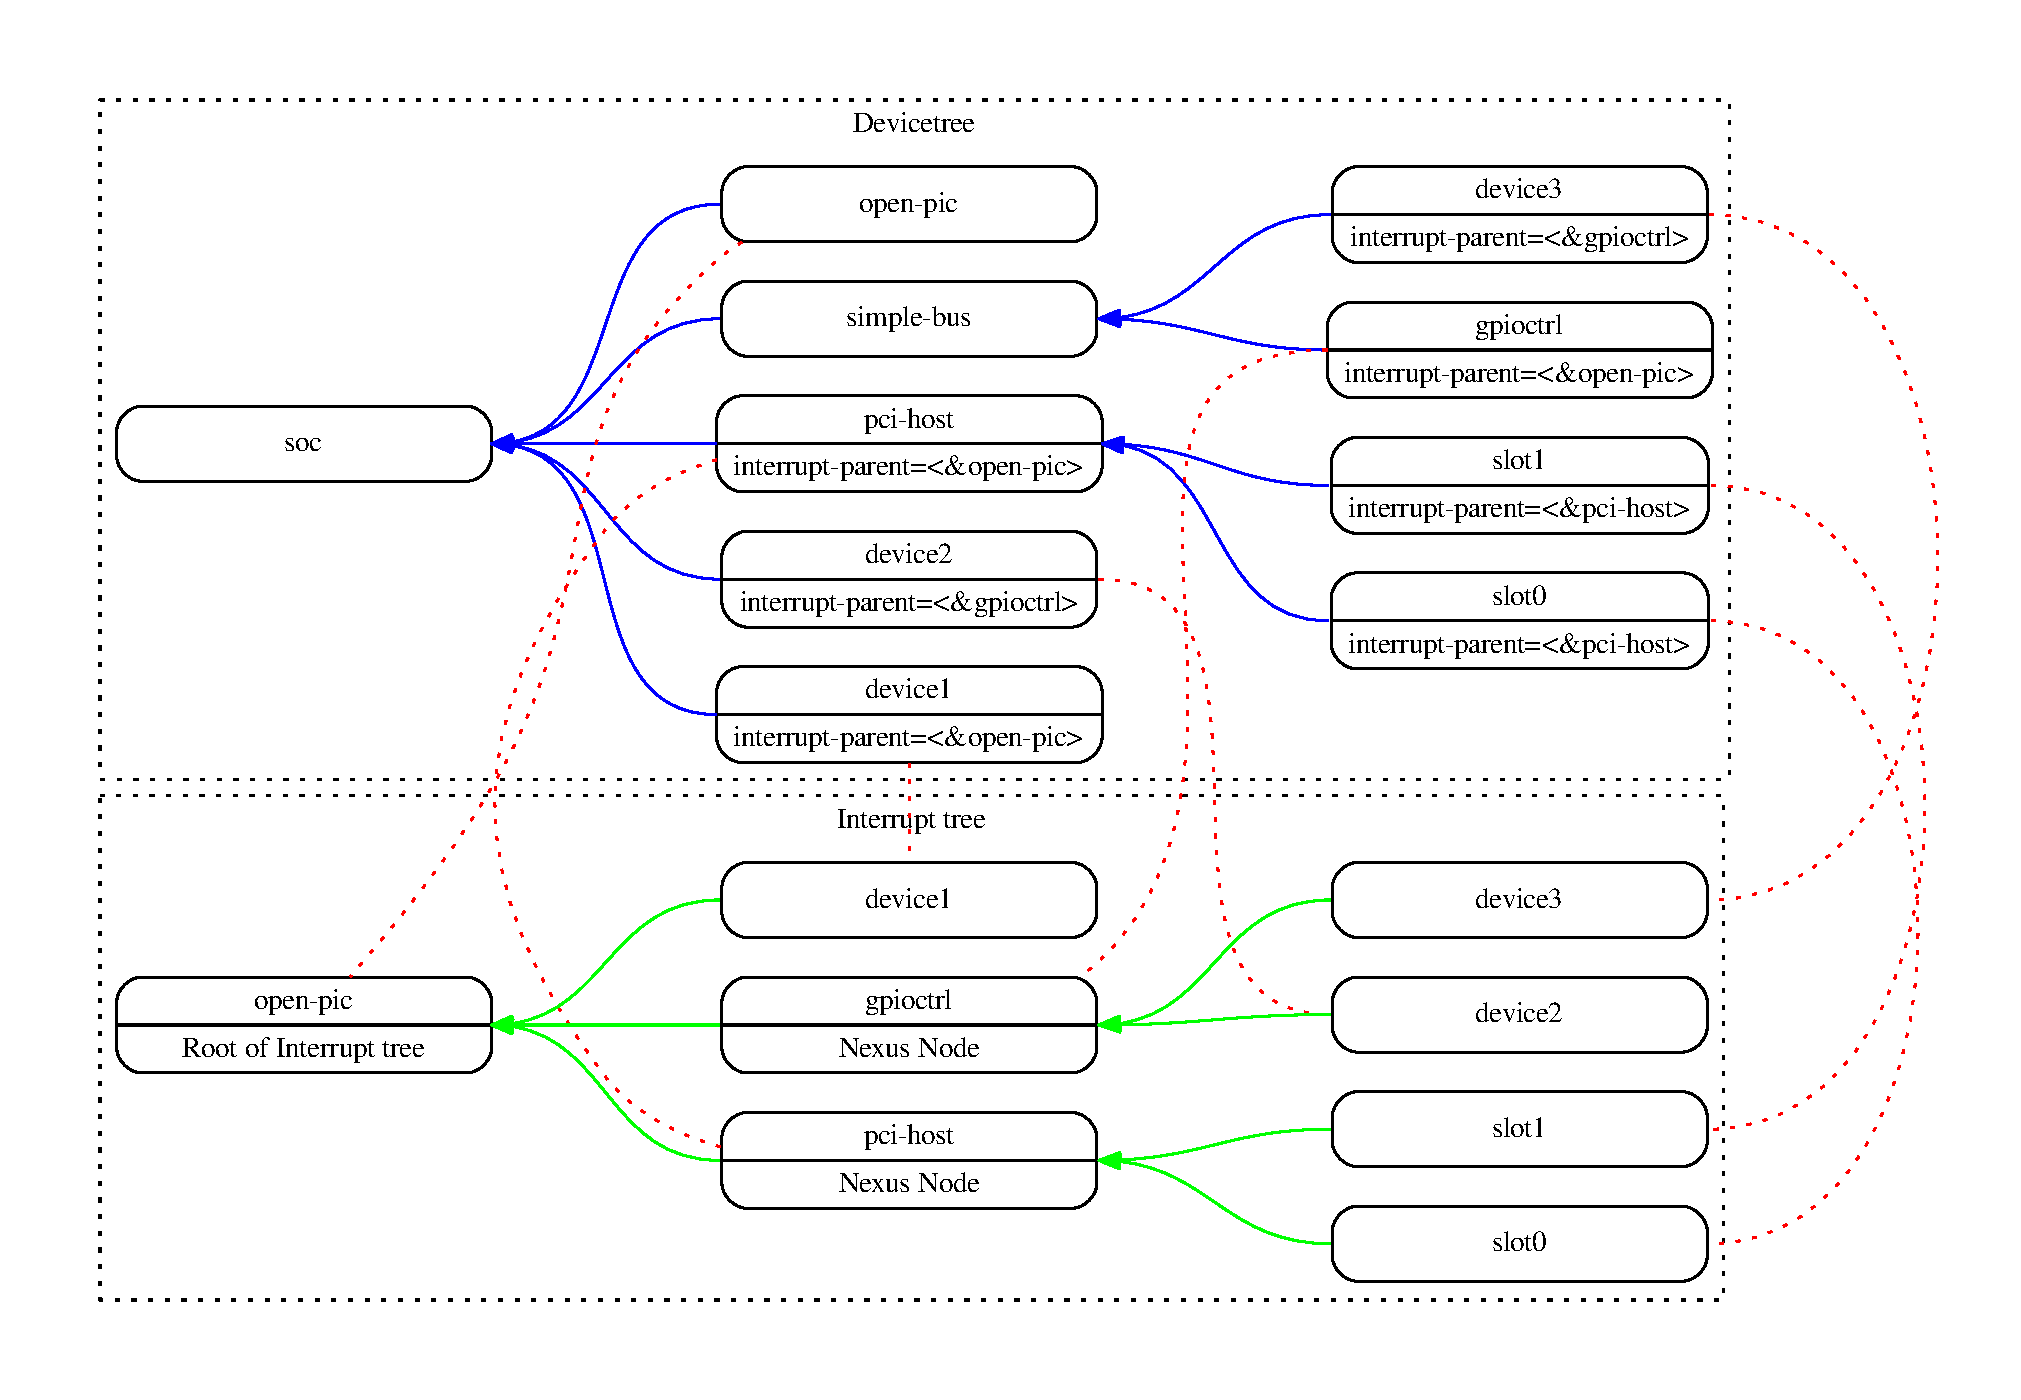
\includegraphics{graphviz-1d3954672eca688030b49a13a35b6714d9abdcd5.pdf}
\caption{Example of the interrupt tree}\label{devicetree-basics:example-interrupt-tree}\label{devicetree-basics:id9}\end{figure}

In the example shown in \hyperref[devicetree-basics:example-interrupt-tree]{Fig. \ref{devicetree-basics:example-interrupt-tree}}:
\begin{itemize}
\item {} 
The \code{open-pic} interrupt controller is the root of the interrupt tree.

\item {} 
The interrupt tree root has three children—devices that route their
interrupts directly to the \code{open-pic}
\begin{itemize}
\item {} 
device1

\item {} 
PCI host controller

\item {} 
GPIO Controller

\end{itemize}

\item {} 
Three interrupt domains exist; one rooted at the \code{open-pic} node,
one at the \code{PCI host bridge} node, and one at the
\code{GPIO Controller} node.

\item {} 
There are two nexus nodes; one at the \code{PCI host bridge} and one at
the \code{GPIO controller}.

\end{itemize}


\subsection{Properties for Interrupt Generating Devices}
\label{devicetree-basics:properties-for-interrupt-generating-devices}

\subsubsection{interrupts}
\label{devicetree-basics:interrupts}
Property: \code{interrupts}

Value type: \code{\textless{}prop-encoded-array\textgreater{}} encoded as arbitrary number of
interrupt specifiers

Description:
\begin{quote}

The \emph{interrupts} property of a device node defines the interrupt or
interrupts that are generated by the device. The value of the
\emph{interrupts} property consists of an arbitrary number of interrupt
specifiers. The format of an interrupt specifier is defined by the
binding of the interrupt domain root.
\end{quote}

Example:
\begin{quote}

A common definition of an interrupt specifier in an open PIC–compatible
interrupt domain consists of two cells; an interrupt number and
level/sense information. See the following example, which defines a
single interrupt specifier, with an interrupt number of 0xA and
level/sense encoding of 8.
\begin{quote}

\code{interrupts = \textless{}0xA 8\textgreater{};}
\end{quote}
\end{quote}


\subsubsection{interrupt-parent}
\label{devicetree-basics:interrupt-parent}
Property: \code{interrupt-parent}

Value type: \code{\textless{}phandle\textgreater{}}

Description:
\begin{quote}

Because the hierarchy of the nodes in the interrupt tree might not match
the devicetree, the \emph{interrupt-parent} property is available to make
the definition of an interrupt parent explicit. The value is the phandle
to the interrupt parent. If this property is missing from a device, its
interrupt parent is assumed to be its devicetree parent.
\end{quote}


\subsection{Properties for Interrupt Controllers}
\label{devicetree-basics:properties-for-interrupt-controllers}

\subsubsection{\#interrupt-cells}
\label{devicetree-basics:interrupt-cells}
Property: \code{\#interrupt-cells}

Value type: \code{\textless{}u32\textgreater{}}

Description:
\begin{quote}

The \emph{\#interrupt-cells} property defines the number of cells required to
encode an interrupt specifier for an interrupt domain.
\end{quote}


\subsubsection{interrupt-controller}
\label{devicetree-basics:interrupt-controller}
Property: \code{interrupt-controller}

Value type: \code{\textless{}empty\textgreater{}}

Description:
\begin{quote}

The presence of an \emph{interrupt-controller} property defines a node as an
interrupt controller node.
\end{quote}


\subsection{Interrupt Nexus Properties}
\label{devicetree-basics:interrupt-nexus-properties}
An interrupt nexus node shall have an \emph{\#interrupt-cells} property.


\subsubsection{interrupt-map}
\label{devicetree-basics:interrupt-map}
Property: \code{interrupt-map}

Value type: \code{\textless{}prop-encoded-array\textgreater{}} encoded as an arbitrary number of
interrupt mapping entries.

Description:
\begin{quote}

An \emph{interrupt-map} is a property on a nexus node that bridges one
interrupt domain with a set of parent interrupt domains and specifies
how interrupt specifiers in the child domain are mapped to their
respective parent domains.

The interrupt map is a table where each row is a mapping entry
consisting of five components: \emph{child unit address}, \emph{child interrupt
specifier}, \emph{interrupt-parent}, \emph{parent unit address}, \emph{parent interrupt
specifier}.
\begin{description}
\item[{child unit address}] \leavevmode
The unit address of the child node being mapped. The number of
32-bit cells required to specify this is described by the
\emph{\#address-cells} property of the bus node on which the child is
located.

\item[{child interrupt specifier}] \leavevmode
The interrupt specifier of the child node being mapped. The number
of 32-bit cells required to specify this component is described by
the \emph{\#interrupt-cells} property of this node—the nexus node
containing the \emph{interrupt-map} property.

\item[{interrupt-parent}] \leavevmode
A single \emph{\textless{}phandle\textgreater{}} value that points to the interrupt parent to
which the child domain is being mapped.

\item[{parent unit address}] \leavevmode
The unit address in the domain of the interrupt parent. The number
of 32-bit cells required to specify this address is described by the
\emph{\#address-cells} property of the node pointed to by the
interrupt-parent field.

\item[{parent interrupt specifier}] \leavevmode
The interrupt specifier in the parent domain. The number of 32-bit
cells required to specify this component is described by the
\emph{\#interrupt-cells} property of this node—the nexus node containing
the \emph{interrupt-map} property.

\end{description}

Lookups are performed on the interrupt mapping table by matching a
unit-address/interrupt specifier pair against the child components in
the interrupt-map. Because some fields in the unit interrupt specifier
may not be relevant, a mask is applied before the lookup is done. This
mask is defined in the \emph{interrupt-map-mask} property (see section
{\hyperref[devicetree\string-basics:sect\string-interrupt\string-map\string-mask]{\crossref{\DUrole{std,std-ref}{2.4.3.2}}}}).

\begin{notice}{note}{Note:}
Both the child node and the interrupt parent node are required to
have \emph{\#address-cells} and \emph{\#interrupt-cells} properties defined. If a
unit address component is not required, \emph{\#address-cells} shall be
explicitly defined to be zero.
\end{notice}
\end{quote}


\subsubsection{interrupt-map-mask}
\label{devicetree-basics:sect-interrupt-map-mask}\label{devicetree-basics:interrupt-map-mask}
Property: \code{interrupt-map-mask}

Value type: \code{\textless{}prop-encoded-array\textgreater{}} encoded as a bit mask

Description:
\begin{quote}

An \emph{interrupt-map-mask} property is specified for a nexus node in the
interrupt tree. This property specifies a mask that is applied to the
incoming unit interrupt specifier being looked up in the table specified
in the \emph{interrupt-map} property.
\end{quote}


\subsubsection{\#interrupt-cells}
\label{devicetree-basics:id2}
Property: \code{\#interrupt-cells}

Value type: \code{\textless{}u32\textgreater{}}

Description:
\begin{quote}

The \emph{\#interrupt-cells} property defines the number of cells required to
encode an interrupt specifier for an interrupt domain.
\end{quote}


\subsection{Interrupt Mapping Example}
\label{devicetree-basics:interrupt-mapping-example}
The following shows the representation of a fragment of a devicetree with
a PCI bus controller and a sample interrupt map for describing the
interrupt routing for two PCI slots (IDSEL 0x11,0x12). The INTA, INTB,
INTC, and INTD pins for slots 1 and 2 are wired to the Open PIC
interrupt controller.
\phantomsection\label{devicetree-basics:example-interrupt-mapping}
\def\SphinxLiteralBlockLabel{\label{devicetree-basics:example-interrupt-mapping}}
\begin{Verbatim}[commandchars=\\\{\}]
soc \PYGZob{}
   compatible = \PYGZdq{}simple\PYGZhy{}bus\PYGZdq{};
   \PYGZsh{}address\PYGZhy{}cells = \PYGZlt{}1\PYGZgt{};
   \PYGZsh{}size\PYGZhy{}cells = \PYGZlt{}1\PYGZgt{};

   open\PYGZhy{}pic \PYGZob{}
      clock\PYGZhy{}frequency = \PYGZlt{}0\PYGZgt{};
      interrupt\PYGZhy{}controller;
      \PYGZsh{}address\PYGZhy{}cells = \PYGZlt{}0\PYGZgt{};
      \PYGZsh{}interrupt\PYGZhy{}cells = \PYGZlt{}2\PYGZgt{};
   \PYGZcb{};

   pci \PYGZob{}
      \PYGZsh{}interrupt\PYGZhy{}cells = \PYGZlt{}1\PYGZgt{};
      \PYGZsh{}size\PYGZhy{}cells = \PYGZlt{}2\PYGZgt{};
      \PYGZsh{}address\PYGZhy{}cells = \PYGZlt{}3\PYGZgt{};
      interrupt\PYGZhy{}map\PYGZhy{}mask = \PYGZlt{}0xf800 0 0 7\PYGZgt{};
      interrupt\PYGZhy{}map = \PYGZlt{}
         /* IDSEL 0x11 \PYGZhy{} PCI slot 1 */
         0x8800 0 0 1 \PYGZam{}open\PYGZhy{}pic 2 1 /* INTA */
         0x8800 0 0 2 \PYGZam{}open\PYGZhy{}pic 3 1 /* INTB */
         0x8800 0 0 3 \PYGZam{}open\PYGZhy{}pic 4 1 /* INTC */
         0x8800 0 0 4 \PYGZam{}open\PYGZhy{}pic 1 1 /* INTD */
         /* IDSEL 0x12 \PYGZhy{} PCI slot 2 */
         0x9000 0 0 1 \PYGZam{}open\PYGZhy{}pic 3 1 /* INTA */
         0x9000 0 0 2 \PYGZam{}open\PYGZhy{}pic 4 1 /* INTB */
         0x9000 0 0 3 \PYGZam{}open\PYGZhy{}pic 1 1 /* INTC */
         0x9000 0 0 4 \PYGZam{}open\PYGZhy{}pic 2 1 /* INTD */
      \PYGZgt{};
   \PYGZcb{};
\PYGZcb{};
\end{Verbatim}
\let\SphinxLiteralBlockLabel\empty

One Open PIC interrupt controller is represented and is identified as an
interrupt controller with an \emph{interrupt-controller} property.

Each row in the interrupt-map table consists of five parts: a child unit
address and interrupt specifier, which is mapped to an \emph{interrupt-parent}
node with a specified parent unit address and interrupt specifier.
\begin{itemize}
\item {} 
For example, the first row of the interrupt-map table specifies the
mapping for INTA of slot 1. The components of that row are shown here

\begin{DUlineblock}{0em}
\item[] child unit address: \code{0x8800 0 0}
\item[] child interrupt specifier: \code{1}
\item[] interrupt parent: \code{\&open-pic}
\item[] parent unit address: (empty because \code{\#address-cells = \textless{}0\textgreater{}} in the
open-pic node)
\item[] parent interrupt specifier: \code{2 1}
\end{DUlineblock}
\begin{itemize}
\item {} 
The child unit address is \code{\textless{}0x8800 0 0\textgreater{}}. This value is encoded
with three 32-bit cells, which is determined by the value of the
\emph{\#address-cells} property (value of 3) of the PCI controller. The
three cells represent the PCI address as described by the binding for
the PCI bus.
\begin{itemize}
\item {} 
The encoding includes the bus number (0x0 \textless{}\textless{} 16), device number
(0x11 \textless{}\textless{} 11), and function number (0x0 \textless{}\textless{} 8).

\end{itemize}

\item {} 
The child interrupt specifier is \code{\textless{}1\textgreater{}}, which specifies INTA as
described by the PCI binding. This takes one 32-bit cell as specified
by the \emph{\#interrupt-cells} property (value of 1) of the PCI
controller, which is the child interrupt domain.

\item {} 
The interrupt parent is specified by a phandle which points to the
interrupt parent of the slot, the Open PIC interrupt controller.

\item {} 
The parent has no unit address because the parent interrupt domain
(the open-pic node) has an \emph{\#address-cells} value of \code{\textless{}0\textgreater{}}.

\item {} 
The parent interrupt specifier is \code{\textless{}2 1\textgreater{}}. The number of cells to
represent the interrupt specifier (two cells) is determined by the
\emph{\#interrupt-cells} property on the interrupt parent, the open-pic
node.
\begin{itemize}
\item {} 
The value \code{\textless{}2 1\textgreater{}} is a value specified by the device binding for
the Open PIC interrupt controller (see section
{\hyperref[device\string-bindings:sect\string-bindings\string-simple\string-bus]{\crossref{\DUrole{std,std-ref}{4.5}}}}). The value \code{\textless{}2\textgreater{}} specifies the
physical interrupt source number on the interrupt controller to
which INTA is wired. The value \code{\textless{}1\textgreater{}} specifies the level/sense
encoding.

\end{itemize}

\end{itemize}

\end{itemize}

In this example, the interrupt-map-mask property has a value of \code{\textless{}0xf800
0 0 7\textgreater{}}. This mask is applied to a child unit interrupt specifier before
performing a lookup in the interruptmap table.

To perform a lookup of the open-pic interrupt source number for INTB for
IDSEL 0x12 (slot 2), function 0x3, the following steps would be
performed:
\begin{itemize}
\item {} 
The child unit address and interrupt specifier form the value
\code{\textless{}0x9300 0 0 2\textgreater{}}.
\begin{itemize}
\item {} 
The encoding of the address includes the bus number (0x0 \textless{}\textless{} 16),
device number (0x12 \textless{}\textless{} 11), and function number (0x3 \textless{}\textless{} 8).

\item {} 
The interrupt specifier is 2, which is the encoding for INTB as
per the PCI binding.

\end{itemize}

\item {} 
The interrupt-map-mask value \code{\textless{}0xf800 0 0 7\textgreater{}} is applied, giving a
result of \code{\textless{}0x9000 0 0 2\textgreater{}}.

\item {} 
That result is looked up in the \emph{interrupt-map} table, which maps to
the parent interrupt specifier \code{\textless{}4 1\textgreater{}}.

\end{itemize}


\chapter{Device Node Requirements}
\label{devicenodes:chapter-device-node-requirements}\label{devicenodes:device-node-requirements}\label{devicenodes::doc}

\section{Base Device Node Types}
\label{devicenodes:base-device-node-types}
The sections that follow specify the requirements for the base set of
device nodes required in an DTSpec-compliant devicetree.

All devicetrees shall have a root node and the following nodes shall be
present at the root of all devicetrees:
\begin{itemize}
\item {} 
One \code{/cpus} node

\item {} 
At least one \code{memory} node

\end{itemize}


\section{Root node}
\label{devicenodes:root-node}
The devicetree has a single root node of which all other device nodes
are descendants. The full path to the root node is \code{/}.


\begin{threeparttable}
\capstart\caption{Root Node Properties}\label{devicenodes:id2}
\begin{tabulary}{\linewidth}{| l c l J |}
\hline
\textsf{\relax 
Property Name
} & \textsf{\relax 
Usage
} & \textsf{\relax 
Value Type
} & \textsf{\relax 
Definition
}\\
\hline
\code{\#address-cells}
 & 
R
 & 
\code{\textless{}u32\textgreater{}}
 & 
Specifies the number of \code{\textless{}u32\textgreater{}} cells to
represent the address in the \code{reg} property in
children of root.
\\
\hline
\code{\#size-cells}
 & 
R
 & 
\code{\textless{}u32\textgreater{}}
 & 
Specifies the number of \code{\textless{}u32\textgreater{}} cells to
represent the size in the \code{reg} property in
children of root.
\\
\hline
\code{model}
 & 
R
 & 
\code{\textless{}string\textgreater{}}
 & 
Specifies a string that uniquely identifies
the model of the system board. The recommended
format is ``manufacturer,model-number''.
\\
\hline
\code{compatible}
 & 
R
 & 
\code{\textless{}stringlist\textgreater{}}
 & 
Specifies a list of platform architectures
with which this platform is compatible. This
property can be used by operating systems in
selecting platform specific code. The
recommended form of the property value is:

\code{"manufacturer,model"}

For example:

\code{compatible = "fsl,mpc8572ds"}
\\
\hline \multicolumn{4}{|l|}{
Usage legend: R=Required, O=Optional, OR=Optional but Recommended, SD=See Definition
}\\
\hline\end{tabulary}

\end{threeparttable}


\begin{notice}{note}{Note:}
All other standard properties (section
{\hyperref[devicetree\string-basics:sect\string-standard\string-properties]{\crossref{\DUrole{std,std-ref}{2.3}}}}) are allowed but are optional.
\end{notice}


\section{\texttt{/aliases} node}
\label{devicenodes:aliases-node}
A devicetree may have an aliases node (\code{/aliases}) that defines one or
more alias properties. The alias node shall be at the root of the devicetree
and have the node name \code{/aliases}.

Each property of the \code{/aliases} node defines an alias. The property name
specifies the alias name. The property value specifies the full path to
a node in the devicetree. For example, the property serial0 =
\code{"/simple-bus@fe000000/serial@llc500"} defines the alias serial0.

Alias names shall be a lowercase text strings of 1 to 31 characters from
the following set of characters.


\begin{threeparttable}
\capstart\caption{Valid characters for alias names}\label{devicenodes:id3}
\begin{tabulary}{\linewidth}{| c p{8cm} |}
\hline
\textsf{\relax 
Character
} & \textsf{\relax 
Description
}\\
\hline
0-9
 & 
digit
\\
\hline
a-z
 & 
lowercase letter
\\
\hline
-
 & 
dash
\\
\hline\end{tabulary}

\end{threeparttable}


An alias value is a device path and is encoded as a string. The value
represents the full path to a node, but the path does not need to refer
to a leaf node.

A client program may use an alias property name to refer to a full
device path as all or part of its string value. A client program, when
considering a string as a device path, shall detect and use the alias.

\textbf{Example}

\begin{Verbatim}[commandchars=\\\{\}]
aliases \PYGZob{}
    serial0 = \PYGZdq{}/simple\PYGZhy{}bus@fe000000/serial@llc500\PYGZdq{};
    ethernet0 = \PYGZdq{}/simple\PYGZhy{}bus@fe000000/ethernet@31c000\PYGZdq{};
\PYGZcb{}
\end{Verbatim}

Given the alias serial0, a client program can look at the aliases node
and determine the alias refers to the device path
\code{/simple-bus@fe000000/serial@llc500}.


\section{\texttt{/memory} node}
\label{devicenodes:memory-node}
A memory device node is required for all devicetrees and describes the
physical memory layout for the system. If a system has multiple ranges
of memory, multiple memory nodes can be created, or the ranges can be
specified in the \emph{reg} property of a single memory node.

The name component of the node name (see section {\hyperref[devicetree\string-basics:sect\string-node\string-names]{\crossref{\DUrole{std,std-ref}{2.2.1}}}})
shall be memory.

The client program may access memory not covered by any memory
reservations (see section {\hyperref[flattened\string-format:sect\string-fdt\string-memory\string-reservation\string-block]{\crossref{\DUrole{std,std-ref}{5.3}}}})
using any storage attributes it chooses. However, before changing the
storage attributes used to access a real page, the client program is
responsible for performing actions required by the architecture and
implementation, possibly including flushing the real page from the
caches. The boot program is responsible for ensuring that, without
taking any action associated with a change in storage attributes, the
client program can safely access all memory (including memory covered by
memory reservations) as WIMG = 0b001x. That is:
\begin{itemize}
\item {} 
not Write Through Required

\item {} 
not Caching Inhibited

\item {} 
Memory Coherence

\item {} 
Required either not Guarded or Guarded

\end{itemize}

If the VLE storage attribute is supported, with VLE=0.


\begin{threeparttable}
\capstart\caption{\texttt{/memory} Node Properties}\label{devicenodes:id4}
\begin{tabulary}{\linewidth}{| l c l J |}
\hline
\textsf{\relax 
Property Name
} & \textsf{\relax 
Usage
} & \textsf{\relax 
Value Type
} & \textsf{\relax 
Definition
}\\
\hline
\code{device\_type}
 & 
R
 & 
\code{\textless{}string\textgreater{}}
 & 
Value shall be ``memory''
\\
\hline
\code{reg}
 & 
R
 & 
\code{\textless{}prop-encoded-array\textgreater{}}
 & 
Consists of an arbitrary number of address and
size pairs that specify the physical address
and size of the memory ranges.
\\
\hline
\code{initial-mapped-area}
 & 
O
 & 
\code{\textless{}prop-encoded-array\textgreater{}}
 & 
Specifies the address and size of the Initial
Mapped Area

Is a prop-encoded-array consisting of a
triplet of (effective address, physical
address, size). The effective and physical
address shall each be 64-bit (\code{\textless{}u64\textgreater{}} value),
and the size shall be 32-bits (\code{\textless{}u32\textgreater{}} value).
\\
\hline \multicolumn{4}{|l|}{
Usage legend: R=Required, O=Optional, OR=Optional but Recommended, SD=See Definition
}\\
\hline\end{tabulary}

\end{threeparttable}


\begin{notice}{note}{Note:}
All other standard properties (section
{\hyperref[devicetree\string-basics:sect\string-standard\string-properties]{\crossref{\DUrole{std,std-ref}{2.3}}}}) are allowed but are optional.
\end{notice}

\textbf{Examples}

Given a 64-bit Power system with the following physical memory layout:
\begin{itemize}
\item {} 
RAM: starting address 0x0, length 0x80000000 (2GB)

\item {} 
RAM: starting address 0x100000000, length 0x100000000 (4GB)

\end{itemize}

Memory nodes could be defined as follows, assuming \code{\#address-cells = \textless{}2\textgreater{}}
and \code{\#size-cells = \textless{}2\textgreater{}}.

\textbf{Example \#1}

\begin{Verbatim}[commandchars=\\\{\}]
memory@0 \PYGZob{}
    device\PYGZus{}type = \PYGZdq{}memory\PYGZdq{};
    reg = \PYGZlt{}0x000000000 0x00000000 0x00000000 0x80000000
           0x000000001 0x00000000 0x00000001 0x00000000\PYGZgt{};
\PYGZcb{};
\end{Verbatim}

\textbf{Example \#2}

\begin{Verbatim}[commandchars=\\\{\}]
memory@0 \PYGZob{}
    device\PYGZus{}type = \PYGZdq{}memory\PYGZdq{};
    reg = \PYGZlt{}0x000000000 0x00000000 0x00000000 0x80000000\PYGZgt{};
\PYGZcb{};
memory@100000000 \PYGZob{}
    device\PYGZus{}type = \PYGZdq{}memory\PYGZdq{};
    reg = \PYGZlt{}0x000000001 0x00000000 0x00000001 0x00000000\PYGZgt{};
\PYGZcb{};
\end{Verbatim}

The \code{reg} property is used to define the address and size of the two
memory ranges. The 2 GB I/O region is skipped. Note that the
\code{\#address-cells} and \code{\#size-cells} properties of the root node specify a
value of 2, which means that two 32-bit cells are required to define the
address and length for the \code{reg} property of the memory node.


\section{\texttt{/chosen} Node}
\label{devicenodes:chosen-node}
The \code{/chosen} node does not represent a real device in the system but
describes parameters chosen or specified by the system firmware at run
time. It shall be a child of the root node.


\begin{threeparttable}
\capstart\caption{\texttt{/chosen} Node Properties}\label{devicenodes:id5}
\begin{tabulary}{\linewidth}{| l c l J |}
\hline
\textsf{\relax 
Property Name
} & \textsf{\relax 
Usage
} & \textsf{\relax 
Value Type
} & \textsf{\relax 
Definition
}\\
\hline
\code{bootargs}
 & 
O
 & 
\code{\textless{}string\textgreater{}}
 & 
A string that specifies the boot arguments for
the client program. The value could
potentially be a null string if no boot
arguments are required.
\\
\hline
\code{stdout-path}
 & 
O
 & 
\code{\textless{}string\textgreater{}}
 & 
A string that specifies the full path to the
node representing the device to be used for
boot console output. If the character '':'' is
present in the value it terminates the path.
The value may be an alias.
If the stdin-path property is not specified,
stdout-path should be assumed to define the
input device.
\\
\hline
\code{stdin-path}
 & 
O
 & 
\code{\textless{}string\textgreater{}}
 & 
A string that specifies the full path to the
node representing the device to be used for
boot console input. If the character '':'' is
present in the value it terminates the path.
The value may be an alias.
\\
\hline \multicolumn{4}{|l|}{
Usage legend: R=Required, O=Optional, OR=Optional but Recommended, SD=See Definition
}\\
\hline\end{tabulary}

\end{threeparttable}


\begin{notice}{note}{Note:}
All other standard properties (section
{\hyperref[devicetree\string-basics:sect\string-standard\string-properties]{\crossref{\DUrole{std,std-ref}{2.3}}}}) are allowed but are optional.
\end{notice}

\textbf{Example}

\begin{Verbatim}[commandchars=\\\{\}]
chosen \PYGZob{}
    bootargs = \PYGZdq{}root=/dev/nfs rw nfsroot=192.168.1.1 console=ttyS0,115200\PYGZdq{};
\PYGZcb{};
\end{Verbatim}

Older versions of devicetrees may be encountered that contain a
deprecated form of the stdout-path property called linux,stdout-path.
For compatibility, a client program might want to support
linux,stdout-path if a stdout-path property is not present. The meaning
and use of the two properties is identical.


\section{\texttt{/cpus} Node Properties}
\label{devicenodes:cpus-node-properties}
A cpus node is required for all devicetrees. It does not represent a
real device in the system, but acts as a container for child cpu nodes
which represent the systems CPUs.


\begin{threeparttable}
\capstart\caption{\texttt{/cpus} Node Properties}\label{devicenodes:id6}
\begin{tabulary}{\linewidth}{| l c l J |}
\hline
\textsf{\relax 
Property Name
} & \textsf{\relax 
Usage
} & \textsf{\relax 
Value Type
} & \textsf{\relax 
Definition
}\\
\hline
\code{\#address-cells}
 & 
R
 & 
\code{\textless{}u32\textgreater{}}
 & 
The value specifies how many cells each
element of the \code{reg} property array takes in
children of this node.
\\
\hline
\code{\#size-cells}
 & 
R
 & 
\code{\textless{}u32\textgreater{}}
 & 
Value shall be 0. Specifies that no size is
required in the \code{reg} property in children of
this node.
\\
\hline \multicolumn{4}{|l|}{
Usage legend: R=Required, O=Optional, OR=Optional but Recommended, SD=See Definition
}\\
\hline\end{tabulary}

\end{threeparttable}


\begin{notice}{note}{Note:}
All other standard properties (section
{\hyperref[devicetree\string-basics:sect\string-standard\string-properties]{\crossref{\DUrole{std,std-ref}{2.3}}}}) are allowed but are optional.
\end{notice}

The cpus node may contain properties that are common across CPU nodes.
See section {\hyperref[devicenodes:sect\string-cpus\string-cpu\string-node\string-properties]{\crossref{\DUrole{std,std-ref}{3.7}}}} for details.

For an example, see section {\hyperref[devicenodes:sect\string-cpu\string-node\string-example]{\crossref{\DUrole{std,std-ref}{3.8.1}}}}.


\section{\texttt{/cpus/cpu*} Node Properties}
\label{devicenodes:sect-cpus-cpu-node-properties}\label{devicenodes:cpus-cpu-node-properties}
A cpu node represents a hardware execution block that is sufficiently
independent that it is capable of running an operating system without
interfering with other CPUs possibly running other operating systems.

Hardware threads that share an MMU would generally be represented under
one cpu node. If other more complex CPU topographies are designed, the
binding for the CPU must describe the topography (e.g. threads that
don’t share an MMU).

CPUs and threads are numbered through a unified number-space that should
match as closely as possible the interrupt controller’s numbering of
CPUs/threads.

Properties that have identical values across CPU nodes may be placed in
the cpus node instead. A client program must first examine a specific
CPU node, but if an expected property is not found then it should look
at the parent cpus node. This results in a less verbose representation
of properties which are identical across all CPUs.

The node name for every cpu node should be \code{cpu}.


\subsection{General Properties of \texttt{/cpus/cpu*} nodes}
\label{devicenodes:general-properties-of-cpus-cpu-nodes}
The following table describes the general properties of CPU nodes. Some
of the properties described in \hyperref[devicenodes:table-cpu-node-props]{Table \ref{devicenodes:table-cpu-node-props}} are select
standard properties with specific applicable detail.

\begin{longtable}{| p{1.5cm} p{1cm} p{2.5cm} p{9.0cm} |}
\caption{\texttt{/cpus/cpu*} Node General Properties}\label{devicenodes:table-cpu-node-props}\\
\hline
\textsf{\relax 
Property Name
} & \textsf{\relax 
Usage
} & \textsf{\relax 
Value Type
} & \textsf{\relax 
Definition
}\\
\hline\endfirsthead

\multicolumn{4}{c}%
{{\tablecontinued{\tablename\ \thetable{} -- continued from previous page}}} \\
\hline
\textsf{\relax 
Property Name
} & \textsf{\relax 
Usage
} & \textsf{\relax 
Value Type
} & \textsf{\relax 
Definition
}\\
\hline\endhead

\hline \multicolumn{4}{|r|}{{\tablecontinued{Continued on next page}}} \\ \hline
\endfoot

\endlastfoot


\code{device\_type}
 & 
\begin{DUlineblock}{0em}
\item[] R
\end{DUlineblock}
 & 
\begin{DUlineblock}{0em}
\item[] \code{\textless{}string\textgreater{}}
\end{DUlineblock}
 & 
Value shall be \code{"cpu"}.
\\
\hline
\code{reg}
 & 
R
 & 
array
 & 
The value of \emph{reg} is a \code{\textless{}prop-encoded-array\textgreater{}}
that defines a unique CPU/thread id for the
CPU/threads represented by the CPU node.

If a CPU supports more than one thread (i.e.
multiple streams of execution) the \emph{reg}
property is an array with 1 element per
thread. The \emph{\#address-cells} on the \code{/cpus} node
specifies how many cells each element of the
array takes. Software can determine the number
of threads by dividing the size of \emph{reg} by
the parent node's \emph{\#address-cells}.

If a CPU/thread can be the target of an
external interrupt the \emph{reg} property value
must be a unique CPU/thread id that is
addressable by the interrupt controller.

If a CPU/thread cannot be the target of an
external interrupt, then \emph{reg} must be unique
and out of bounds of the range addressed by
the interrupt controller

If a CPU/thread's PIR is modifiable, a client
program should modify PIR to match the \emph{reg}
property value. If PIR cannot be modified and
the PIR value is distinct from the interrupt
controller numberspace, the CPUs binding may
define a binding-specific representation of
PIR values if desired.
\\
\hline
\code{clock-frequency}
 & 
\begin{DUlineblock}{0em}
\item[] R
\end{DUlineblock}
 & 
\begin{DUlineblock}{0em}
\item[] array
\end{DUlineblock}
 & 
Specifies the current clock speed of the CPU
in Hertz. The value is a \code{\textless{}prop-encoded-array\textgreater{}}
in one of two forms:
\begin{itemize}
\item {} 
A 32-bit integer consisting of one \code{\textless{}u32\textgreater{}}
specifying the frequency.

\item {} 
A 64-bit integer represented as a \code{\textless{}u64\textgreater{}}
specifying the frequency.

\end{itemize}
\\
\hline
\code{timebase-frequency}
 & 
\begin{DUlineblock}{0em}
\item[] R
\end{DUlineblock}
 & 
\begin{DUlineblock}{0em}
\item[] array
\end{DUlineblock}
 & 
Specifies the current frequency at which the
timebase and decrementer registers are updated
(in Hertz). The value is a
\textless{}prop-encoded-array\textgreater{} in one of two forms:
\begin{itemize}
\item {} 
A 32-bit integer consisting of one \code{\textless{}u32\textgreater{}}
specifying the frequency.

\item {} 
A 64-bit integer represented as a \code{\textless{}u64\textgreater{}}.

\end{itemize}
\\
\hline
\code{status}
 & 
SD
 & 
\code{\textless{}string\textgreater{}}
 & 
A standard property describing the state of a
CPU. This property shall be present for nodes
representing CPUs in a symmetric
multiprocessing (SMP) configuration. For a CPU
node the meaning of the \code{"okay"} and
\code{"disabled"} values are as follows:
\begin{description}
\item[{\code{"okay"} :}] \leavevmode
The CPU is running.

\item[{\code{"disabled"} :}] \leavevmode
The CPU is in a quiescent state.

\end{description}

A quiescent CPU is in a state where it cannot
interfere with the normal operation of other
CPUs, nor can its state be affected by the
normal operation of other running CPUs, except
by an explicit method for enabling or
reenabling the quiescent CPU (see the
enable-method property).

In particular, a running CPU shall be able to
issue broadcast TLB invalidates without
affecting a quiescent CPU.

Examples: A quiescent CPU could be in a spin
loop, held in reset, and electrically isolated
from the system bus or in another
implementation dependent state.
\\
\hline
\code{enable-method}
 & 
\begin{DUlineblock}{0em}
\item[] SD
\end{DUlineblock}
 & 
\begin{DUlineblock}{0em}
\item[] \code{\textless{}stringlist\textgreater{}}
\end{DUlineblock}
 & 
Describes the method by which a CPU in a
disabled state is enabled. This property is
required for CPUs with a status property with
a value of \code{"disabled"}. The value consists of
one or more strings that define the method to
release this CPU. If a client program
recognizes any of the methods, it may use it.
The value shall be one of the following:
\begin{description}
\item[{\code{"spin-table"} :}] \leavevmode
The CPU is enabled with the
spin table method defined in the DTSpec.

\item[{\code{"{[}vendor{]},{[}method{]}"} :}] \leavevmode
Implementation dependent string that
describes the method by which a CPU is
released from a \code{"disabled"} state. The
required format is: \code{"{[}vendor{]},{[}method{]}"},
where vendor is a string describing the name of
the manufacturer and method is a string
describing the vendorspecific mechanism.

\end{description}

Example: \code{"fsl,MPC8572DS"}

\begin{notice}{note}{Note:}
Other methods may be added to later
revisions of the DTSpec specification.
\end{notice}
\\
\hline
\code{cpu-release-addr}
 & 
\begin{DUlineblock}{0em}
\item[] SD
\end{DUlineblock}
 & 
\begin{DUlineblock}{0em}
\item[] \code{\textless{}u64\textgreater{}}
\end{DUlineblock}
 & 
The cpu-release-addr property is required for
cpu nodes that have an enable-method property
value of \code{"spin-table"}. The value specifies the
physical address of a spin table entry that
releases a secondary CPU from its spin loop.
\\
\hline \multicolumn{4}{|l|}{
Usage legend: R=Required, O=Optional, OR=Optional but Recommended, SD=See Definition
}\\
\hline\end{longtable}


\begin{notice}{note}{Note:}
All other standard properties (section
{\hyperref[devicetree\string-basics:sect\string-standard\string-properties]{\crossref{\DUrole{std,std-ref}{2.3}}}}) are allowed but are optional.
\end{notice}

\begin{longtable}{| p{1.5cm} p{1cm} p{2.5cm} p{9.0cm} |}
\caption{\texttt{/cpus/cpu*} Node Power ISA Properties}\\
\hline
\textsf{\relax 
Property Name
} & \textsf{\relax 
Usage
} & \textsf{\relax 
Value Type
} & \textsf{\relax 
Definition
}\\
\hline\endfirsthead

\multicolumn{4}{c}%
{{\tablecontinued{\tablename\ \thetable{} -- continued from previous page}}} \\
\hline
\textsf{\relax 
Property Name
} & \textsf{\relax 
Usage
} & \textsf{\relax 
Value Type
} & \textsf{\relax 
Definition
}\\
\hline\endhead

\hline \multicolumn{4}{|r|}{{\tablecontinued{Continued on next page}}} \\ \hline
\endfoot

\endlastfoot


\code{power-isa-version}
 & 
\begin{DUlineblock}{0em}
\item[] O
\end{DUlineblock}
 & 
\begin{DUlineblock}{0em}
\item[] \code{\textless{}string\textgreater{}}
\end{DUlineblock}
 & 
A string that specifies the numerical portion
of the Power ISA version string. For example,
for an implementation complying with Power ISA
Version 2.06, the value of this property would
be \code{"2.06"}.
\\
\hline
\code{power-isa-*}
 & 
\begin{DUlineblock}{0em}
\item[] O
\end{DUlineblock}
 & 
\begin{DUlineblock}{0em}
\item[] \code{\textless{}empty\textgreater{}}
\end{DUlineblock}
 & 
If the \code{power-isa-version} property exists, then
for each category from the Categories section
of Book I of the Power ISA version indicated,
the existence of a property named
\code{power-isa-{[}CAT{]}}, where \code{{[}CAT{]}} is the
abbreviated category name with all uppercase
letters converted to lowercase, indicates that
the category is supported by the
implementation.

For example, if the power-isa-version property
exists and its value is \code{"2.06"} and the
power-isa-e.hv property exists, then the
implementation supports
{[}Category:Embedded.Hypervisor{]} as defined in
Power ISA Version 2.06.
\\
\hline
\code{cache-op-block-size}
 & 
\begin{DUlineblock}{0em}
\item[] SD
\end{DUlineblock}
 & 
\begin{DUlineblock}{0em}
\item[] \code{\textless{}u32\textgreater{}}
\end{DUlineblock}
 & 
Specifies the block size in bytes upon which
cache block instructions operate (e.g., dcbz).
Required if different than the L1 cache block
size.
\\
\hline
\code{reservation-granule-size}
 & 
\begin{DUlineblock}{0em}
\item[] SD
\end{DUlineblock}
 & 
\begin{DUlineblock}{0em}
\item[] \code{\textless{}u32\textgreater{}}
\end{DUlineblock}
 & 
Specifies the reservation granule size
supported by this processor in bytes.
\\
\hline
\code{mmu-type}
 & 
O
 & 
\code{\textless{}string\textgreater{}}
 & 
Specifies the CPU’s MMU type.

Valid values are shown below:
\begin{itemize}
\item {} 
\code{"mpc8xx"}

\item {} 
\code{"ppc40x"}

\item {} 
\code{"ppc440"}

\item {} 
\code{"ppc476"}

\item {} 
\code{"power-embedded"}

\item {} 
\code{"powerpc-classic"}

\item {} 
\code{"power-server-stab"}

\item {} 
\code{"power-server-slb"}

\item {} 
\code{"none"}

\end{itemize}
\\
\hline \multicolumn{4}{|l|}{
Usage legend: R=Required, O=Optional, OR=Optional but Recommended, SD=See Definition
}\\
\hline\end{longtable}


\begin{notice}{note}{Note:}
All other standard properties (section
{\hyperref[devicetree\string-basics:sect\string-standard\string-properties]{\crossref{\DUrole{std,std-ref}{2.3}}}}) are allowed but are optional.
\end{notice}

Older versions of devicetree may be encountered that contain a
bus-frequency property on CPU nodes. For compatibility, a client-program
might want to support bus-frequency. The format of the value is
identical to that of clock-frequency. The recommended practice is to
represent the frequency of a bus on the bus node using a clock-frequency
property.


\subsection{TLB Properties}
\label{devicenodes:tlb-properties}
The following properties of a cpu node describe the translate look-aside
buffer in the processor’s MMU.


\begin{threeparttable}
\capstart\caption{\texttt{/cpu/cpu*} Node Power ISA TLB Properties}\label{devicenodes:id9}
\begin{tabulary}{\linewidth}{| l c l J |}
\hline
\textsf{\relax 
Property Name
} & \textsf{\relax 
Usage
} & \textsf{\relax 
Value Type
} & \textsf{\relax 
Definition
}\\
\hline
\code{tlb-split}
 & 
SD
 & 
\code{\textless{}empty\textgreater{}}
 & 
If present specifies that the TLB has a split
configuration, with separate TLBs for
instructions and data. If absent, specifies
that the TLB has a unified configuration.
Required for a CPU with a TLB in a split
configuration.
\\
\hline
\code{tlb-size}
 & 
SD
 & 
\code{\textless{}u32\textgreater{}}
 & 
Specifies the number of entries in the TLB.
Required for a CPU with a unified TLB for
instruction and data addresses.
\\
\hline
\code{tlb-sets}
 & 
SD
 & 
\code{\textless{}u32\textgreater{}}
 & 
Specifies the number of associativity sets in
the TLB. Required for a CPU with a unified TLB
for instruction and data addresses.
\\
\hline
\code{d-tlb-size}
 & 
SD
 & 
\code{\textless{}u32\textgreater{}}
 & 
Specifies the number of entries in the data
TLB. Required for a CPU with a split TLB
configuration.
\\
\hline
\code{d-tlb-sets}
 & 
SD
 & 
\code{\textless{}u32\textgreater{}}
 & 
Specifies the number of associativity sets in
the data TLB. Required for a CPU with a split
TLB configuration.
\\
\hline
\code{i-tlb-size}
 & 
SD
 & 
\code{\textless{}u32\textgreater{}}
 & 
Specifies the number of entries in the
instruction TLB. Required for a CPU with a
split TLB configuration.
\\
\hline
\code{i-tlb-sets}
 & 
SD
 & 
\code{\textless{}u32\textgreater{}}
 & 
Specifies the number of associativity sets in
the instruction TLB. Required for a CPU with a
split TLB configuration.
\\
\hline \multicolumn{4}{|l|}{
Usage legend: R=Required, O=Optional, OR=Optional but Recommended, SD=See Definition
}\\
\hline\end{tabulary}

\end{threeparttable}


\begin{notice}{note}{Note:}
All other standard properties (section
{\hyperref[devicetree\string-basics:sect\string-standard\string-properties]{\crossref{\DUrole{std,std-ref}{2.3}}}}) are allowed but are optional.
\end{notice}


\subsection{Internal (L1) Cache Properties}
\label{devicenodes:internal-l1-cache-properties}
The following properties of a cpu node describe the processor’s internal
(L1) cache.


\begin{threeparttable}
\capstart\caption{\texttt{/cpu/cpu*} Node Power ISA Cache Properties}\label{devicenodes:id10}
\begin{tabulary}{\linewidth}{| l c l J |}
\hline
\textsf{\relax 
Property Name
} & \textsf{\relax 
Usage
} & \textsf{\relax 
Value Type
} & \textsf{\relax 
Definition
}\\
\hline
\code{cache-unified}
 & 
SD
 & 
\code{\textless{}empty\textgreater{}}
 & 
If present, specifies the cache has a unified
organization. If not present, specifies that
the cache has a Harvard architecture with
separate caches for instructions and data.
\\
\hline
\code{cache-size}
 & 
SD
 & 
\code{\textless{}u32\textgreater{}}
 & 
Specifies the size in bytes of a unified
cache. Required if the cache is unified
(combined instructions and data).
\\
\hline
\code{cache-sets}
 & 
SD
 & 
\code{\textless{}u32\textgreater{}}
 & 
Specifies the number of associativity sets in
a unified cache. Required if the cache is
unified (combined instructions and data)
\\
\hline
\code{cache-block-size}
 & 
SD
 & 
\code{\textless{}u32\textgreater{}}
 & 
Specifies the block size in bytes of a unified
cache. Required if the processor has a unified
cache (combined instructions and data)
\\
\hline
\code{cache-line-size}
 & 
SD
 & 
\code{\textless{}u32\textgreater{}}
 & 
Specifies the line size in bytes of a unified
cache, if different than the cache block size
Required if the processor has a unified cache
(combined instructions and data).
\\
\hline
\code{i-cache-size}
 & 
SD
 & 
\code{\textless{}u32\textgreater{}}
 & 
Specifies the size in bytes of the instruction
cache. Required if the cpu has a separate
cache for instructions.
\\
\hline
\code{i-cache-sets}
 & 
SD
 & 
\code{\textless{}u32\textgreater{}}
 & 
Specifies the number of associativity sets in
the instruction cache. Required if the cpu has
a separate cache for instructions.
\\
\hline
\code{i-cache-block-size}
 & 
SD
 & 
\code{\textless{}u32\textgreater{}}
 & 
Specifies the block size in bytes of the
instruction cache. Required if the cpu has a
separate cache for instructions.
\\
\hline
\code{i-cache-line-size}
 & 
SD
 & 
\code{\textless{}u32\textgreater{}}
 & 
Specifies the line size in bytes of the
instruction cache, if different than the cache
block size. Required if the cpu has a separate
cache for instructions.
\\
\hline
\code{d-cache-size}
 & 
SD
 & 
\code{\textless{}u32\textgreater{}}
 & 
Specifies the size in bytes of the data cache.
Required if the cpu has a separate cache for
data.
\\
\hline
\code{d-cache-sets}
 & 
SD
 & 
\code{\textless{}u32\textgreater{}}
 & 
Specifies the number of associativity sets in
the data cache. Required if the cpu has a
separate cache for data.
\\
\hline
\code{d-cache-block-size}
 & 
SD
 & 
\code{\textless{}u32\textgreater{}}
 & 
Specifies the block size in bytes of the data
cache. Required if the cpu has a separate
cache for data.
\\
\hline
\code{d-cache-line-size}
 & 
SD
 & 
\code{\textless{}u32\textgreater{}}
 & 
Specifies the line size in bytes of the data
cache, if different than the cache block size.
Required if the cpu has a separate cache for
data.
\\
\hline
\code{next-level-cache}
 & 
SD
 & 
\code{\textless{}phandle\textgreater{}}
 & 
If present, indicates that another level of
cache exists. The value is the phandle of the
next level of cache. The phandle value type is
fully described in section {\hyperref[devicetree\string-basics:sect\string-standard\string-properties\string-phandle]{\crossref{\DUrole{std,std-ref}{2.3.3}}}}.
\\
\hline \multicolumn{4}{|l|}{
Usage legend: R=Required, O=Optional, OR=Optional but Recommended, SD=See Definition
}\\
\hline\end{tabulary}

\end{threeparttable}


\begin{notice}{note}{Note:}
All other standard properties (section
{\hyperref[devicetree\string-basics:sect\string-standard\string-properties]{\crossref{\DUrole{std,std-ref}{2.3}}}}) are allowed but are optional.
\end{notice}

Older versions of devicetrees may be encountered that contain a
deprecated form of the next-level-cache property called \code{l2-cache}.
For compatibility, a client-program may wish to support \code{l2-cache}
if a next-level-cache property is not present.
The meaning and use of the two properties is identical.


\subsection{Example}
\label{devicenodes:sect-cpu-node-example}\label{devicenodes:example}
Here is an example of a \code{/cpus} node with one child cpu node:

\begin{Verbatim}[commandchars=\\\{\}]
cpus \PYGZob{}
    \PYGZsh{}address\PYGZhy{}cells = \PYGZlt{}1\PYGZgt{};
    \PYGZsh{}size\PYGZhy{}cells = \PYGZlt{}0\PYGZgt{};
    cpu@0 \PYGZob{}
        device\PYGZus{}type = \PYGZdq{}cpu\PYGZdq{};
        reg = \PYGZlt{}0\PYGZgt{};
        d\PYGZhy{}cache\PYGZhy{}block\PYGZhy{}size = \PYGZlt{}32\PYGZgt{}; // L1 \PYGZhy{} 32 bytes
        i\PYGZhy{}cache\PYGZhy{}block\PYGZhy{}size = \PYGZlt{}32\PYGZgt{}; // L1 \PYGZhy{} 32 bytes
        d\PYGZhy{}cache\PYGZhy{}size = \PYGZlt{}0x8000\PYGZgt{}; // L1, 32K
        i\PYGZhy{}cache\PYGZhy{}size = \PYGZlt{}0x8000\PYGZgt{}; // L1, 32K
        timebase\PYGZhy{}frequency = \PYGZlt{}82500000\PYGZgt{}; // 82.5 MHz
        clock\PYGZhy{}frequency = \PYGZlt{}825000000\PYGZgt{}; // 825 MHz
    \PYGZcb{};
\PYGZcb{};
\end{Verbatim}


\section{Multi-level and Shared Cache Nodes (\texttt{/cpus/cpu*/l?-cache})}
\label{devicenodes:multi-level-and-shared-cache-nodes-cpus-cpu-l-cache}
Processors and systems may implement additional levels of cache hierarchy.
For example, second-level (L2) or third-level (L3) caches.
These caches can potentially be tightly integrated to the CPU or
possibly shared between multiple CPUs.

A device node with a compatible value of \code{"cache"} describes these types
of caches.

The cache node shall define a phandle property, and all cpu nodes or
cache nodes that are associated with or share the cache each shall
contain a next-level-cache property that specifies the phandle to the
cache node.

A cache node may be represented under a CPU node or any other
appropriate location in the devicetree.

Multiple-level and shared caches are represented with the properties in
Table 3-9. The L1 cache properties are described in Table 3-8.


\begin{threeparttable}
\capstart\caption{\texttt{/cpu/cpu*/l?-cache} Node Power ISA Multiple-level and Shared Cache Properties}\label{devicenodes:id11}
\begin{tabulary}{\linewidth}{| l c l J |}
\hline
\textsf{\relax 
Property Name
} & \textsf{\relax 
Usage
} & \textsf{\relax 
Value Type
} & \textsf{\relax 
Definition
}\\
\hline
\code{compatible}
 & 
R
 & 
\code{\textless{}string\textgreater{}}
 & 
A standard property. The value shall include
the string \code{"cache"}.
\\
\hline
\code{cache-level}
 & 
R
 & 
\code{\textless{}u32\textgreater{}}
 & 
Specifies the level in the cache hierarchy.
For example, a level 2 cache has a value of 2.
\\
\hline \multicolumn{4}{|l|}{
Usage legend: R=Required, O=Optional, OR=Optional but Recommended, SD=See Definition
}\\
\hline\end{tabulary}

\end{threeparttable}


\begin{notice}{note}{Note:}
All other standard properties (section
{\hyperref[devicetree\string-basics:sect\string-standard\string-properties]{\crossref{\DUrole{std,std-ref}{2.3}}}}) are allowed but are optional.
\end{notice}


\subsection{Example}
\label{devicenodes:id1}
See the following example of a devicetree representation of two CPUs,
each with their own on-chip L2 and a shared L3.

\begin{Verbatim}[commandchars=\\\{\}]
cpus \PYGZob{}
    \PYGZsh{}address\PYGZhy{}cells = \PYGZlt{}1\PYGZgt{};
    \PYGZsh{}size\PYGZhy{}cells = \PYGZlt{}0\PYGZgt{};
    cpu@0 \PYGZob{}
        device\PYGZus{}type = \PYGZdq{}cpu\PYGZdq{};
        reg = \PYGZlt{}0\PYGZgt{};
        cache\PYGZhy{}unified;
        cache\PYGZhy{}size = \PYGZlt{}0x8000\PYGZgt{}; // L1, 32KB
        cache\PYGZhy{}block\PYGZhy{}size = \PYGZlt{}32\PYGZgt{};
        timebase\PYGZhy{}frequency = \PYGZlt{}82500000\PYGZgt{}; // 82.5 MHz
        next\PYGZhy{}level\PYGZhy{}cache = \PYGZlt{}\PYGZam{}L2\PYGZus{}0\PYGZgt{}; // phandle to L2

        L2\PYGZus{}0:l2\PYGZhy{}cache \PYGZob{}
            compatible = \PYGZdq{}cache\PYGZdq{};
            cache\PYGZhy{}unified;
            cache\PYGZhy{}size = \PYGZlt{}0x40000\PYGZgt{}; // 256 KB

            cache\PYGZhy{}sets = \PYGZlt{}1024\PYGZgt{};
            cache\PYGZhy{}block\PYGZhy{}size = \PYGZlt{}32\PYGZgt{};
            cache\PYGZhy{}level = \PYGZlt{}2\PYGZgt{};
            next\PYGZhy{}level\PYGZhy{}cache = \PYGZlt{}\PYGZam{}L3\PYGZgt{}; // phandle to L3

            L3:l3\PYGZhy{}cache \PYGZob{}
                compatible = \PYGZdq{}cache\PYGZdq{};
                cache\PYGZhy{}unified;
                cache\PYGZhy{}size = \PYGZlt{}0x40000\PYGZgt{}; // 256 KB
                cache\PYGZhy{}sets = \PYGZlt{}0x400\PYGZgt{}; // 1024
                cache\PYGZhy{}block\PYGZhy{}size =
                cache\PYGZhy{}level = \PYGZlt{}3\PYGZgt{};
            \PYGZcb{};
        \PYGZcb{};
    \PYGZcb{};

    cpu@1 \PYGZob{}
        device\PYGZus{}type = \PYGZdq{}cpu\PYGZdq{};
        reg = \PYGZlt{}0\PYGZgt{};
        cache\PYGZhy{}unified;
        cache\PYGZhy{}block\PYGZhy{}size = \PYGZlt{}32\PYGZgt{};
        cache\PYGZhy{}size = \PYGZlt{}0x8000\PYGZgt{}; // L1, 32KB
        timebase\PYGZhy{}frequency = \PYGZlt{}82500000\PYGZgt{}; // 82.5 MHz
        clock\PYGZhy{}frequency = \PYGZlt{}825000000\PYGZgt{}; // 825 MHz
        cache\PYGZhy{}level = \PYGZlt{}2\PYGZgt{};
        next\PYGZhy{}level\PYGZhy{}cache = \PYGZlt{}\PYGZam{}L2\PYGZus{}1\PYGZgt{}; // phandle to L2
        L2\PYGZus{}1:l2\PYGZhy{}cache \PYGZob{}
            compatible = \PYGZdq{}cache\PYGZdq{};
            cache\PYGZhy{}unified;
            cache\PYGZhy{}size = \PYGZlt{}0x40000\PYGZgt{}; // 256 KB
            cache\PYGZhy{}sets = \PYGZlt{}0x400\PYGZgt{}; // 1024
            cache\PYGZhy{}line\PYGZhy{}size = \PYGZlt{}32\PYGZgt{} // 32 bytes
            next\PYGZhy{}level\PYGZhy{}cache = \PYGZlt{}\PYGZam{}L3\PYGZgt{}; // phandle to L3
        \PYGZcb{};
    \PYGZcb{};
\PYGZcb{};
\end{Verbatim}


\chapter{Device Bindings}
\label{device-bindings::doc}\label{device-bindings:device-bindings}\label{device-bindings:chapter-device-bindings}
This chapter contains requirements, known as bindings, for how specific
types and classes of devices are represented in the devicetree. The
compatible property of a device node describes the specific binding (or
bindings) to which the node complies.

Bindings may be defined as extensions of other each. For example a new
bus type could be defined as an extension of the simple-bus binding. In
this case, the compatible property would contain several strings
identifying each binding—from the most specific to the most general (see
section {\hyperref[devicetree\string-basics:sect\string-standard\string-properties\string-compatible]{\crossref{\DUrole{std,std-ref}{2.3.1}}}}, compatible).


\section{Binding Guidelines}
\label{device-bindings:binding-guidelines}

\subsection{General Principles}
\label{device-bindings:general-principles}
When creating a new devicetree representation for a device, a binding
should be created that fully describes the required properties and value
of the device. This set of properties shall be sufficiently descriptive
to provide device drivers with needed attributes of the device.

Some recommended practices include:
\begin{enumerate}
\item {} 
Define a compatible string using the conventions described in section
{\hyperref[devicetree\string-basics:sect\string-standard\string-properties\string-compatible]{\crossref{\DUrole{std,std-ref}{2.3.1}}}}.

\item {} 
Use the standard properties (defined in sections
{\hyperref[devicetree\string-basics:sect\string-standard\string-properties]{\crossref{\DUrole{std,std-ref}{2.3}}}} and {\hyperref[devicetree\string-basics:sect\string-interrupts]{\crossref{\DUrole{std,std-ref}{2.4}}}}) as
applicable for the new device. This usage typically includes the
\code{reg} and \code{interrupts} properties at a minimum.

\item {} 
Use the conventions specified in section {\hyperref[device\string-bindings:chapter\string-device\string-bindings]{\crossref{\DUrole{std,std-ref}{4}}}}
(Device Bindings) if the new device fits into one the DTSpec defined
device classes.

\item {} 
Use the miscellaneous property conventions specified in section
{\hyperref[device\string-bindings:sect\string-misc\string-properties]{\crossref{\DUrole{std,std-ref}{4.1.2}}}}, if applicable.

\item {} 
If new properties are needed by the binding, the recommended format
for property names is: \code{"\textless{}company\textgreater{},\textless{}property-name\textgreater{}"}, where \code{\textless{}company\textgreater{}}
is an OUI or short unique string like a stock ticker that identifies
the creator of the binding.

Example: \code{"ibm,ppc-interrupt-server\#s"}

\end{enumerate}


\subsection{Miscellaneous Properties}
\label{device-bindings:sect-misc-properties}\label{device-bindings:miscellaneous-properties}
This section defines a list of helpful properties that might be
applicable to many types of devices and device classes. They are defined
here to facilitate standardization of names and usage.


\subsubsection{\texttt{clock-frequency} Property}
\label{device-bindings:clock-frequency-property}

\begin{threeparttable}
\capstart\caption{\texttt{clock-frequency} Property}\label{device-bindings:id3}
\begin{tabulary}{\linewidth}{| l J |}
\hline
\textsf{\relax 
Property
} & \textsf{\relax 
\code{clock-frequency}
}\\
\hline
Value type
 & 
\code{\textless{}prop-encoded-array\textgreater{}}
\\
\hline
Description
 & 
Specifies the frequency of a clock in Hz. The value is a
\code{\textless{}prop-encoded-array\textgreater{}} in one of two forms:

a 32-bit integer consisting of one \code{\textless{}u32\textgreater{}} specifying the
frequency

a 64-bit integer represented as a \code{\textless{}u64\textgreater{}} specifying the
frequency
\\
\hline\end{tabulary}

\end{threeparttable}



\subsubsection{\texttt{reg-shift} Property}
\label{device-bindings:reg-shift-property}

\begin{threeparttable}
\capstart\caption{\texttt{reg-shift} Property}\label{device-bindings:id4}
\begin{tabulary}{\linewidth}{| l J |}
\hline
\textsf{\relax 
Property
} & \textsf{\relax 
\code{reg-shift}
}\\
\hline
Value type
 & 
\code{\textless{}u32\textgreater{}}
\\
\hline
Description
 & 
The \code{reg-shift} property provides a mechanism to represent
devices that are identical in most respects except for the
number of bytes between registers. The \code{reg-shift} property
specifies in bytes how far the discrete device registers are
separated from each other. The individual register location
is calculated by using following formula: ``registers address''
\textless{}\textless{} reg-shift. If unspecified, the default value is 0.

For example, in a system where 16540 UART registers are
located at addresses 0x0, 0x4, 0x8, 0xC, 0x10, 0x14, 0x18,
and 0x1C, a \code{reg-shift = \textless{}2\textgreater{}}
property would be used to specify register locations.
\\
\hline\end{tabulary}

\end{threeparttable}



\subsubsection{\texttt{label} Property}
\label{device-bindings:label-property}

\begin{threeparttable}
\capstart\caption{\texttt{label} Property}\label{device-bindings:id5}
\begin{tabulary}{\linewidth}{| l J |}
\hline
\textsf{\relax 
Property
} & \textsf{\relax 
\code{label}
}\\
\hline
Value type
 & 
\code{\textless{}string\textgreater{}}
\\
\hline
Descriptio
 & 
The label property defines a human readable string describing
a device. The binding for a given device specifies the exact
meaning of the property for that device.
\\
\hline\end{tabulary}

\end{threeparttable}



\section{Serial devices}
\label{device-bindings:serial-devices}

\subsection{Serial Class Binding}
\label{device-bindings:serial-class-binding}
The class of serial devices consists of various types of point to point
serial line devices. Examples of serial line devices include the 8250
UART, 16550 UART, HDLC device, and BISYNC device. In most cases hardware
compatible with the RS-232 standard fit into the serial device class.

I$^{\text{2}}$C and SPI (Serial Peripheral Interface) devices shall not
be represented as serial port devices because they have their own
specific representation.


\subsubsection{\texttt{clock-frequency} Property}
\label{device-bindings:id1}

\begin{threeparttable}
\capstart\caption{\texttt{clock-frequecy} Property}\label{device-bindings:id6}
\begin{tabulary}{\linewidth}{| l J |}
\hline
\textsf{\relax 
Property
} & \textsf{\relax 
\code{clock-frequency}
}\\
\hline
Value type
 & 
\code{\textless{}u32\textgreater{}}
\\
\hline
Description
 & 
Specifies the frequency in Hertz of the baud rate generator's
input clock.
\\
\hline
Example
 & 
\code{clock-frequency = \textless{}100000000\textgreater{};}
\\
\hline\end{tabulary}

\end{threeparttable}



\subsubsection{\texttt{current-speed} Property}
\label{device-bindings:current-speed-property}

\begin{threeparttable}
\capstart\caption{\texttt{current-speed} Property}\label{device-bindings:id7}
\begin{tabulary}{\linewidth}{l J}
\hline
\textsf{\relax 
Property
} & \textsf{\relax 
\code{current-speed}
}\\
\hline
Value type
 & 
\code{\textless{}u32\textgreater{}}
\\
\hline
Description
 & 
Specifies the current speed of a serial device in bits per
second. A boot program should set this property if it has
initialized the serial device.
\\
\hline
Example
 & 
115,200 Baud: \code{current-speed = \textless{}115200\textgreater{};}
\\
\hline\end{tabulary}

\end{threeparttable}



\subsection{National Semiconductor 16450/16550 Compatible UART Requirements}
\label{device-bindings:national-semiconductor-16450-16550-compatible-uart-requirements}
Serial devices compatible to the National Semiconductor 16450/16550 UART
(Universal Asynchronous Receiver Transmitter) should be represented in
the devicetree using following properties.


\begin{threeparttable}
\capstart\caption{ns16550 UART Properties}\label{device-bindings:id8}
\begin{tabulary}{\linewidth}{l c l J}
\hline
\textsf{\relax 
Property Name
} & \textsf{\relax 
Usage
} & \textsf{\relax 
Value Type
} & \textsf{\relax 
Definition
}\\
\hline
\code{compatible}
 & 
R
 & 
\textless{}string list\textgreater{}
 & 
Value shall include ``ns16550''.
\\
\hline
\code{clock-frequency}
 & 
R
 & 
\code{\textless{}u32\textgreater{}}
 & 
Specifies the frequency (in Hz) of the baud
rate generator’s input clock
\\
\hline
\code{current-speed}
 & 
OR
 & 
\code{\textless{}u32\textgreater{}}
 & 
Specifies current serial device speed in bits
per second
\\
\hline
\code{reg}
 & 
R
 & 
\code{\textless{}prop encoded
array\textgreater{}}
 & 
Specifies the physical address of the
registers device within the address space of
the parent bus
\\
\hline
\code{interrupts}
 & 
OR
 & 
\code{\textless{}prop encoded
array\textgreater{}}
 & 
Specifies the interrupts generated by this
device. The value of the interrupts property
consists of one or more interrupt specifiers.
The format of an interrupt specifier is
defined by the binding document describing the
node’s interrupt parent.
\\
\hline
\code{reg-shift}
 & 
O
 & 
\code{\textless{}u32\textgreater{}}
 & 
Specifies in bytes how far the discrete device
registers are separated from each other. The
individual register location is calculated by
using following formula: \code{"registers address"
\textless{}\textless{} reg-shift}. If unspecified, the default
value is 0.
\\
\hline
\code{virtual-reg}
 & 
SD
 & 
\code{\textless{}u32\textgreater{}}
or
\code{\textless{}u64\textgreater{}}
 & 
See section {\hyperref[devicetree\string-basics:sect\string-standard\string-properties\string-virtual\string-reg]{\crossref{\DUrole{std,std-ref}{2.3.7}}}}.
Specifies an effective address that maps to the
first physical address specified in the \code{reg}
property. This property is required if this
device node is the system’s console.
\\
\hline \multicolumn{4}{|l|}{
Usage legend: R=Required, O=Optional, OR=Optional but Recommended, SD=See Definition
}\\
\hline\end{tabulary}

\end{threeparttable}


\begin{notice}{note}{Note:}
All other standard properties (section
{\hyperref[devicetree\string-basics:sect\string-standard\string-properties]{\crossref{\DUrole{std,std-ref}{2.3}}}}) are allowed but are optional.
\end{notice}


\section{Network devices}
\label{device-bindings:network-devices}
Network devices are packet oriented communication devices. Devices in
this class are assumed to implement the data link layer (layer 2) of the
seven-layer OSI model and use Media Access Control (MAC) addresses.
Examples of network devices include Ethernet, FDDI, 802.11, and
Token-Ring.


\subsection{Network Class Binding}
\label{device-bindings:network-class-binding}

\subsubsection{\texttt{address-bits} Property}
\label{device-bindings:address-bits-property}

\begin{threeparttable}
\capstart\caption{\texttt{address-bits} Property}\label{device-bindings:id9}
\begin{tabulary}{\linewidth}{| l J |}
\hline
\textsf{\relax 
Property
} & \textsf{\relax 
\code{address-bits}
}\\
\hline
Value type
 & 
\code{\textless{}u32\textgreater{}}
\\
\hline
Description
 & 
Specifies number of address bits required to address the
device described by this node. This property specifies number
of bits in MAC address. If unspecified, the default value is 48.
\\
\hline
Example
 & 
\code{address-bits = \textless{}48\textgreater{};}
\\
\hline\end{tabulary}

\end{threeparttable}



\subsubsection{\texttt{local-mac-address} Property}
\label{device-bindings:local-mac-address-property}

\begin{threeparttable}
\capstart\caption{\texttt{local-mac-address} Property}\label{device-bindings:id10}
\begin{tabulary}{\linewidth}{| l J |}
\hline
\textsf{\relax 
Property
} & \textsf{\relax 
\code{local-mac-address}
}\\
\hline
Value type
 & 
\code{\textless{}prop-encoded-array\textgreater{}} encoded as an array of hex numbers
\\
\hline
Description
 & 
Specifies MAC address that was assigned to the network device
described by the node containing this property.
\\
\hline
Example
 & 
\code{local-mac-address = {[} 0x00 0x00 0x12 0x34 0x56 0x78{]};}
\\
\hline\end{tabulary}

\end{threeparttable}



\subsubsection{\texttt{mac-address} Property}
\label{device-bindings:mac-address-property}

\begin{threeparttable}
\capstart\caption{\texttt{mac-address} Property}\label{device-bindings:id11}
\begin{tabulary}{\linewidth}{| l J |}
\hline
\textsf{\relax 
Property
} & \textsf{\relax 
\code{mac-address}
}\\
\hline
Value type
 & 
\code{\textless{}prop-encoded-array\textgreater{}} encoded as an array of hex numbers
\\
\hline
Description
 & 
Specifies the MAC address that was last used by the boot
program. This property should be used in cases where the MAC
address assigned to the device by the boot program is
different from the local-mac-address property. This property
shall be used only if the value differs from
local-mac-address property value.
\\
\hline
Example
 & 
\code{mac-address = {[} 0x01 0x02 0x03 0x04 0x05 0x06 {]};}
\\
\hline\end{tabulary}

\end{threeparttable}



\subsubsection{\texttt{max-frame-size} Property}
\label{device-bindings:max-frame-size-property}

\begin{threeparttable}
\capstart\caption{\texttt{max-frame-size} Property}\label{device-bindings:id12}
\begin{tabulary}{\linewidth}{| l J |}
\hline
\textsf{\relax 
Property
} & \textsf{\relax 
\code{max-frame-size}
}\\
\hline
Value type
 & 
\code{\textless{}u32\textgreater{}}
\\
\hline
Descriptio
 & 
Specifies maximum packet length in bytes that the physical
interface can send and receive.
\\
\hline
Example
 & 
\code{max-frame-size = \textless{}1518\textgreater{};}
\\
\hline\end{tabulary}

\end{threeparttable}



\subsection{Ethernet specific considerations}
\label{device-bindings:ethernet-specific-considerations}
Network devices based on the IEEE 802.3 collections of LAN standards
(collectively referred to as Ethernet) may be represented in the devicetree
using following properties, in addition to properties specified of
the network device class.

The properties listed in this section augment the properties listed in
the network device class.


\subsubsection{\texttt{max-speed} Property}
\label{device-bindings:max-speed-property}

\begin{threeparttable}
\capstart\caption{\texttt{max-speed} Property}\label{device-bindings:id13}
\begin{tabulary}{\linewidth}{| l J |}
\hline
\textsf{\relax 
Property
} & \textsf{\relax 
\code{max-speed}
}\\
\hline
Value type
 & 
\code{\textless{}u32\textgreater{}}
\\
\hline
Description
 & 
Specifies maximum speed (specified in megabits per second)
supported the device.
\\
\hline
Example
 & 
\code{max-speed = \textless{}1000\textgreater{};}
\\
\hline\end{tabulary}

\end{threeparttable}



\subsubsection{\texttt{phy-connection-type} Property}
\label{device-bindings:phy-connection-type-property}

\begin{threeparttable}
\capstart\caption{\texttt{phy-connection-type} Property}\label{device-bindings:id14}
\begin{tabulary}{\linewidth}{| l J |}
\hline
\textsf{\relax 
Property
} & \textsf{\relax 
\code{phy-connection-type}
}\\
\hline
Value type
 & 
\code{\textless{}string\textgreater{}}
\\
\hline
Description
 & 
Specifies interface type between the Ethernet device and a
physical layer (PHY) device. The value of this property is
specific to the implementation.

Recommended values are shown in the following table.
\\
\hline
Example
 & 
\code{phy-connection-type = "mii";}
\\
\hline\end{tabulary}

\end{threeparttable}



\begin{threeparttable}
\capstart\caption{Defined values for the \texttt{phy-connection-type} Property}\label{device-bindings:id15}
\begin{tabulary}{\linewidth}{| l J |}
\hline
\textsf{\relax 
Connection type
} & \textsf{\relax 
Value
}\\
\hline
Media Independent Interface
 & 
\code{mii}
\\
\hline
Reduced Media Independent Interface
 & 
\code{rmii}
\\
\hline
Gigabit Media Independent Interface
 & 
\code{gmii}
\\
\hline
Reduced Gigabit Media Independent
 & 
\code{rgmii}
\\
\hline
rgmii with internal delay
 & 
\code{rgmii-id}
\\
\hline
rgmii with internal delay on TX only
 & 
\code{rgmii-txid}
\\
\hline
rgmii with internal delay on RX only
 & 
\code{rgmii-rxid}
\\
\hline
Ten Bit Interface
 & 
\code{tbi}
\\
\hline
Reduced Ten Bit Interface
 & 
\code{rtbi}
\\
\hline
Serial Media Independent Interface
 & 
\code{smii}
\\
\hline
Serial Gigabit Media Independent Interface
 & 
\code{sgmii}
\\
\hline
Reverse Media Independent Interface
 & 
\code{rev-mii}
\\
\hline
10 Gigabits Media Independent Interface
 & 
\code{xgmii}
\\
\hline
Multimedia over Coaxial
 & 
\code{moca}
\\
\hline
Quad Serial Gigabit Media Independent Interface
 & 
\code{qsgmii}
\\
\hline\end{tabulary}

\end{threeparttable}



\subsubsection{\texttt{phy-handle} Property}
\label{device-bindings:phy-handle-property}

\begin{threeparttable}
\capstart\caption{\texttt{phy-handle} Property}\label{device-bindings:id16}
\begin{tabulary}{\linewidth}{| l J |}
\hline
\textsf{\relax 
Property
} & \textsf{\relax 
\code{phy-handle}
}\\
\hline
Value type
 & 
\code{\textless{}phandle\textgreater{}}
\\
\hline
Description
 & 
Specifies a reference to a node representing a physical layer
(PHY) device connected to this Ethernet device. This property
is required in case where the Ethernet device is connected a
physical layer device.
\\
\hline
Example
 & 
\code{phy-handle = \textless{}\&PHY0\textgreater{};}
\\
\hline\end{tabulary}

\end{threeparttable}



\section{Power ISA Open PIC Interrupt Controllers}
\label{device-bindings:power-isa-open-pic-interrupt-controllers}
This section specifies the requirements for representing Open PIC
compatible interrupt controllers. An Open PIC interrupt controller
implements the Open PIC architecture (developed jointly by AMD and
Cyrix) and specified in The Open Programmable Interrupt Controller (PIC)
Register Interface Specification Revision 1.2 \phantomsection\label{device-bindings:id2}{\hyperref[references:b18]{\crossref{{[}b18{]}}}}.

Interrupt specifiers in an Open PIC interrupt domain are encoded with
two cells. The first cell defines the interrupt number. The second cell
defines the sense and level information.

Sense and level information shall be encoded as follows in interrupt
specifiers:
\begin{quote}

\begin{Verbatim}[commandchars=\\\{\}]
0 = low to high edge sensitive type enabled
1 = active low level sensitive type enabled
2 = active high level sensitive type enabled
3 = high to low edge sensitive type enabled
\end{Verbatim}
\end{quote}


\begin{threeparttable}
\capstart\caption{Open-PIC properties}\label{device-bindings:id17}
\begin{tabulary}{\linewidth}{| l c l J |}
\hline
\textsf{\relax 
Property Name
} & \textsf{\relax 
Usage
} & \textsf{\relax 
Value Type
} & \textsf{\relax 
Definition
}\\
\hline
\code{compatible}
 & 
R
 & 
\code{\textless{}string\textgreater{}}
 & 
Value shall include \code{"open-pic"}
\\
\hline
\code{reg}
 & 
R
 & 
\code{\textless{}prop encoded
array\textgreater{}}
 & 
Specifies the physical address of the
registers device within the address space of
the parent bus
\\
\hline
\code{interrupt-controller}
 & 
R
 & 
\code{\textless{}empty\textgreater{}}
 & 
Specifies that this node is an interrupt controller
\\
\hline
\code{\#interrupt-cells}
 & 
R
 & 
\code{\textless{}u32\textgreater{}}
 & 
Shall be 2.
\\
\hline
\code{\#address-cells}
 & 
R
 & 
\code{\textless{}u32\textgreater{}}
 & 
Shall be 0.
\\
\hline \multicolumn{4}{|l|}{
Usage legend: R=Required, O=Optional, OR=Optional but Recommended, SD=See Definition
}\\
\hline\end{tabulary}

\end{threeparttable}


\begin{notice}{note}{Note:}
All other standard properties (section
{\hyperref[devicetree\string-basics:sect\string-standard\string-properties]{\crossref{\DUrole{std,std-ref}{2.3}}}}) are allowed but are optional.
\end{notice}


\section{\texttt{simple-bus} Compatible Value}
\label{device-bindings:simple-bus-compatible-value}\label{device-bindings:sect-bindings-simple-bus}
System-on-a-chip processors may have an internal I/O bus that cannot be
probed for devices. The devices on the bus can be accessed directly
without additional configuration required. This type of bus is
represented as a node with a compatible value of ``simple-bus''.


\begin{threeparttable}
\capstart\caption{\texttt{simple-bus} Compatible Node Properties}\label{device-bindings:id18}
\begin{tabulary}{\linewidth}{| l c l J |}
\hline
\textsf{\relax 
Property Name
} & \textsf{\relax 
Usage
} & \textsf{\relax 
Value Type
} & \textsf{\relax 
Definition
}\\
\hline
\code{compatible}
 & 
R
 & 
\code{\textless{}string\textgreater{}}
 & 
Value shall include ``simple-bus''.
\\
\hline
\code{ranges}
 & 
R
 & 
\code{\textless{}prop encoded
array\textgreater{}}
 & 
This property represents the mapping between
parent address to child address spaces (see
section {\hyperref[devicetree\string-basics:sect\string-standard\string-properties\string-ranges]{\crossref{\DUrole{std,std-ref}{2.3.8}}}},
ranges).
\\
\hline \multicolumn{4}{|l|}{
Usage legend: R=Required, O=Optional, OR=Optional but Recommended, SD=See Definition
}\\
\hline\end{tabulary}

\end{threeparttable}



\chapter{Flat Devicetree Physical Structure}
\label{flattened-format:flat-devicetree-physical-structure}\label{flattened-format::doc}\label{flattened-format:chapter-fdt-structure}
With the exception of platforms using IEEE1275 Open Firmware {[}IEEE1275{]}, the
devicetree data is contained within a single single, linear, pointerless data
structure known as the flattened devicetree or devicetree blob.

This data structure consists of a small header
(see section {\hyperref[flattened\string-format:sect\string-fdt\string-header]{\crossref{\DUrole{std,std-ref}{5.2}}}}),
followed by three variable sized sections:
the memory reservation block (see section {\hyperref[flattened\string-format:sect\string-fdt\string-memory\string-reservation\string-block]{\crossref{\DUrole{std,std-ref}{5.3}}}}),
the structure block (see secton {\hyperref[flattened\string-format:sect\string-fdt\string-structure\string-block]{\crossref{\DUrole{std,std-ref}{5.4}}}}),
and the strings block (see section {\hyperref[flattened\string-format:sect\string-fdt\string-strings\string-block]{\crossref{\DUrole{std,std-ref}{5.5}}}}).
These should be present in the flattened devicetree in that order.
Thus, the devicetree structure as a whole, when loaded into memory at address,
will resemble the diagram in \hyperref[flattened-format:figure-device-tree-structure]{Fig. \ref{flattened-format:figure-device-tree-structure}}
(lower addresses are at the top of the diagram).
\begin{figure}[htbp]
\centering
\capstart

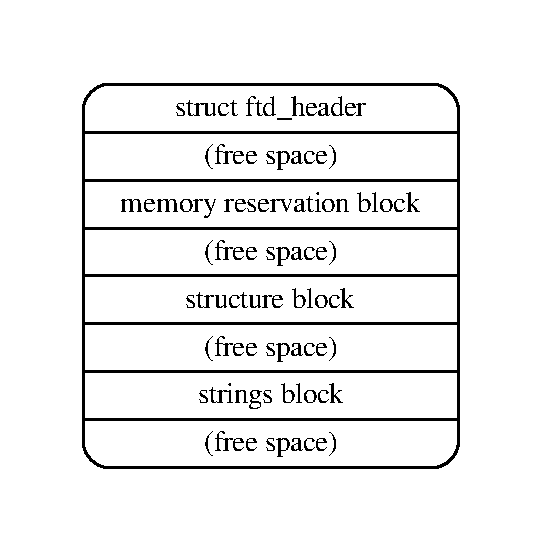
\includegraphics{graphviz-23a197b43ca822bb92fb1a341bdd04b0845caa29.pdf}
\caption{Devicetree .dtb Structure}\label{flattened-format:figure-device-tree-structure}\label{flattened-format:id1}\end{figure}

The (free space) sections may not be present, though in some cases they
might be required to satisfy the alignment constraints of the individual
blocks (see section {\hyperref[flattened\string-format:sect\string-fdt\string-alignment]{\crossref{\DUrole{std,std-ref}{5.6}}}}).


\section{Versioning}
\label{flattened-format:sect-fdt-versioning}\label{flattened-format:versioning}
Several versions of the flattened devicetree structure have been defined since
the original definition of the format. Fields in the header give the version,
so that the client program can determine if the devicetree is encoded in a
compatible format.

This document describes only version 17 of the format. DTSpec compliant boot
programs shall provide a devicetree of version 17 or later, and should provide
a devicetree of a version that is backwards compatible with version 16.
DTSpec compliant client programs shall accept devicetrees of any version
backwards compatible with version 17 and may accept other versions as well.

\begin{notice}{note}{Note:}
The version is with respect to the binary structure of the device
tree, not its content.
\end{notice}


\section{Header}
\label{flattened-format:sect-fdt-header}\label{flattened-format:header}
The layout of the header for the devicetree is defined by the following
C structure. All the header fields are 32-bit integers, stored in
big-endian format.

\textbf{Flattened Devicetree Header Fields}

\begin{Verbatim}[commandchars=\\\{\}]
struct fdt\PYGZus{}header \PYGZob{}
    uint32\PYGZus{}t magic;
    uint32\PYGZus{}t totalsize;
    uint32\PYGZus{}t off\PYGZus{}dt\PYGZus{}struct;
    uint32\PYGZus{}t off\PYGZus{}dt\PYGZus{}strings;
    uint32\PYGZus{}t off\PYGZus{}mem\PYGZus{}rsvmap;
    uint32\PYGZus{}t version;
    uint32\PYGZus{}t last\PYGZus{}comp\PYGZus{}version;
    uint32\PYGZus{}t boot\PYGZus{}cpuid\PYGZus{}phys;
    uint32\PYGZus{}t size\PYGZus{}dt\PYGZus{}strings;
    uint32\PYGZus{}t size\PYGZus{}dt\PYGZus{}struct;
\PYGZcb{};
\end{Verbatim}
\begin{description}
\item[{\code{magic}}] \leavevmode
This field shall contain the value 0xd00dfeed (big-endian).

\item[{\code{totalsize}}] \leavevmode
This field shall contain the total size of the devicetree data
structure. This size shall encompass all sections of the structure:
the header, the memory reservation block, structure block and
strings block, as well as any free space gaps between the blocks or
after the final block.

\item[{\code{off\_dt\_struct}}] \leavevmode
This field shall contain the offset in bytes of the structure block
(see section {\hyperref[flattened\string-format:sect\string-fdt\string-structure\string-block]{\crossref{\DUrole{std,std-ref}{5.4}}}}) from the beginning of the header.

\item[{\code{off\_dt\_strings}}] \leavevmode
This field shall contain the offset in bytes of the strings block
(see section {\hyperref[flattened\string-format:sect\string-fdt\string-strings\string-block]{\crossref{\DUrole{std,std-ref}{5.5}}}}) from the beginning of the header.

\item[{\code{off\_mem\_rsvmap}}] \leavevmode
This field shall contain the offset in bytes of the memory
reservation block (see section {\hyperref[flattened\string-format:sect\string-fdt\string-memory\string-reservation\string-block]{\crossref{\DUrole{std,std-ref}{5.3}}}})
from the beginning of the header.

\item[{\code{version}}] \leavevmode
This field shall contain the version of the devicetree data
structure. The version is 17 if using the structure as defined in
this document. An DTSpec boot program may provide the devicetree of
a later version, in which case this field shall contain the version
number defined in whichever later document gives the details of that
version.

\item[{\code{last\_comp\_version}}] \leavevmode
This field shall contain the lowest version of the devicetree data
structure with which the version used is backwards compatible. So,
for the structure as defined in this document (version 17), this
field shall contain 16 because version 17 is backwards compatible
with version 16, but not earlier versions. As per section
{\hyperref[flattened\string-format:sect\string-fdt\string-versioning]{\crossref{\DUrole{std,std-ref}{5.1}}}}, a DTSpec boot program should provide a
devicetree in a format which is backwards compatible with version
16, and thus this field shall always contain 16.

\item[{\code{boot\_cpuid\_phys}}] \leavevmode
This field shall contain the physical ID of the system’s boot CPU.
It shall be identical to the physical ID given in the \code{reg} property
of that CPU node within the devicetree.

\item[{\code{size\_dt\_strings}}] \leavevmode
This field shall contain the length in bytes of the strings block
section of the devicetree blob.

\item[{\code{size\_dt\_struct}}] \leavevmode
This field shall contain the length in bytes of the structure block
section of the devicetree blob.

\end{description}


\section{Memory Reservation Block}
\label{flattened-format:memory-reservation-block}\label{flattened-format:sect-fdt-memory-reservation-block}

\subsection{Purpose}
\label{flattened-format:purpose}
The \emph{memory reservation block} provides the client program with a list
of areas in physical memory which are \emph{reserved}; that is, which shall
not be used for general memory allocations. It is used to protect vital
data structures from being overwritten by the client program. For
example, on some systems with an IOMMU, the TCE (translation control
entry) tables initialized by a DTSpec boot program would need to be
protected in this manner. Likewise, any boot program code or data used
during the client program’s runtime would need to be reserved (e.g.,
RTAS on Open Firmware platforms). DTSpec does not require the boot
program to provide any such runtime components, but it does not prohibit
implementations from doing so as an extension.

More specifically, a client program shall not access memory in a
reserved region unless other information provided by the boot program
explicitly indicates that it shall do so. The client program may then
access the indicated section of the reserved memory in the indicated
manner. Methods by which the boot program can indicate to the client
program specific uses for reserved memory may appear in this document,
in optional extensions to it, or in platform-specific documentation.

The reserved regions supplied by a boot program may, but are not
required to, encompass the devicetree blob itself. The client program
shall ensure that it does not overwrite this data structure before it is
used, whether or not it is in the reserved areas.

Any memory that is declared in a memory node and is accessed by the boot
program or caused to be accessed by the boot program after client entry
must be reserved. Examples of this type of access include (e.g.,
speculative memory reads through a non-guarded virtual page).

This requirement is necessary because any memory that is not reserved
may be accessed by the client program with arbitrary storage attributes.

Any accesses to reserved memory by or caused by the boot program must be
done as not Caching Inhibited and Memory Coherence Required (i.e., WIMG
= 0bx01x), and additionally for Book III-S implementations as not Write
Through Required (i.e., WIMG = 0b001x). Further, if the VLE storage
attribute is supported, all accesses to reserved memory must be done as
VLE=0.

This requirement is necessary because the client program is permitted to
map memory with storage attributes specified as not Write Through
Required, not Caching Inhibited, and Memory Coherence Required (i.e.,
WIMG = 0b001x), and VLE=0 where supported. The client program may use
large virtual pages that contain reserved memory. However, the client
program may not modify reserved memory, so the boot program may perform
accesses to reserved memory as Write Through Required where conflicting
values for this storage attribute are architecturally permissible.


\subsection{Format}
\label{flattened-format:format}
The memory reservation block consists of a list of pairs of 64-bit
big-endian integers, each pair being represented by the following C
structure.

\begin{Verbatim}[commandchars=\\\{\}]
struct fdt\PYGZus{}reserve\PYGZus{}entry \PYGZob{}
    uint64\PYGZus{}t address;
    uint64\PYGZus{}t size;
\PYGZcb{};
\end{Verbatim}

Each pair gives the physical address and size of a reserved memory
region. These given regions shall not overlap each other. The list of
reserved blocks shall be terminated with an entry where both address and
size are equal to 0. Note that the address and size values are always
64-bit. On 32-bit CPUs the upper 32-bits of the value are ignored.

Each uint64\_t in the memory reservation block, and thus the memory
reservation block as a whole, shall be located at an 8-byte aligned
offset from the beginning of the devicetree blob (see section
{\hyperref[flattened\string-format:sect\string-fdt\string-alignment]{\crossref{\DUrole{std,std-ref}{5.6}}}}).


\section{Structure Block}
\label{flattened-format:sect-fdt-structure-block}\label{flattened-format:structure-block}
The structure block describes the structure and contents of the devicetree
itself. It is composed of a sequence of tokens with data, as
described in 0. These are organized into a linear tree structure, as
described in 0.

Each token in the structure block, and thus the structure block itself,
shall be located at a 4-byte aligned offset from the beginning of the
devicetree blob (see {\hyperref[flattened\string-format:sect\string-fdt\string-alignment]{\crossref{\DUrole{std,std-ref}{5.6}}}}).


\subsection{Lexical structure}
\label{flattened-format:lexical-structure}\label{flattened-format:sect-fdt-lexical-structure}
The structure block is composed of a sequence of pieces, each beginning
with a token, that is, a bigendian 32-bit integer. Some tokens are
followed by extra data, the format of which is determined by the token
value. All tokens shall be aligned on a 32-bit boundary, which may
require padding bytes (with a value of 0x0) to be inserted after the
previous token’s data.

The five token types are as follows:
\begin{description}
\item[{\code{FDT\_BEGIN\_NODE} (0x00000001)}] \leavevmode
The FDT\_BEGIN\_NODE token marks the beginning of a node’s
representation. It shall be followed by the node’s unit name as
extra data. The name is stored as a null-terminated string, and
shall include the unit address (see section {\hyperref[devicetree\string-basics:sect\string-node\string-names]{\crossref{\DUrole{std,std-ref}{2.2.1}}}}), if any.
The node name is followed by zeroed padding bytes, if necessary for
alignment, and then the next token, which may be any token except
FDT\_END.

\item[{\code{FDT\_END\_NODE} (0x00000002)}] \leavevmode
The FDT\_END\_NODE token marks the end of a node’s representation.
This token has no extra data; so it is followed immediately by the
next token, which may be any token except FDT\_PROP.

\item[{\code{FDT\_PROP} (0x00000003)}] \leavevmode
The FDT\_PROP token marks the beginning of the representation of one
property in the devicetree. It shall be followed by extra data
describing the property. This data consists first of the property’s
length and name represented as the following C structure:

\begin{Verbatim}[commandchars=\\\{\}]
struct \PYGZob{}
    uint32\PYGZus{}t len;
    uint32\PYGZus{}t nameoff;
\PYGZcb{}
\end{Verbatim}

Both the fields in this structure are 32-bit big-endian integers.
\begin{itemize}
\item {} 
len gives the length of the property’s value in bytes (which may be
zero, indicating an empty property, see section {\hyperref[devicetree\string-basics:sect\string-property\string-values]{\crossref{\DUrole{std,std-ref}{2.2.4.2}}}}).

\item {} 
nameoff gives an offset into the strings block
(see section {\hyperref[flattened\string-format:sect\string-fdt\string-strings\string-block]{\crossref{\DUrole{std,std-ref}{5.5}}}})
at which the property’s name is stored as a null-terminated string.

\end{itemize}

After this structure, the property’s value is given as a byte string of
length len. This value is followed by zeroed padding bytes (if
necessary) to align to the next 32-bit boundary and then the next token,
which may be any token except FDT\_END.

\item[{\code{FDT\_NOP} (0x00000004)}] \leavevmode
The FDT\_NOP token will be ignored by any program parsing the device
tree. This token has no extra data; so it is followed immediately by
the next token, which can be any valid token. A property or node
definition in the tree can be overwritten with FDT\_NOP tokens to
remove it from the tree without needing to move other sections of
the tree’s representation in the devicetree blob.

\item[{\code{FDT\_END} (0x00000009)}] \leavevmode
The FDT\_END token marks the end of the structure block. There shall
be only one FDT\_END token, and it shall be the last token in the
structure block. It has no extra data; so the byte immediately after
the FDT\_END token has offset from the beginning of the structure
block equal to the value of the size\_dt\_struct field in the device
tree blob header.

\end{description}


\subsection{Tree structure}
\label{flattened-format:tree-structure}
The devicetree structure is represented as a linear tree: the
representation of each node begins with an FDT\_BEGIN\_NODE token and
ends with an FDT\_END\_NODE token. The node’s properties and subnodes
(if any) are represented before the FDT\_END\_NODE, so that the
FDT\_BEGIN\_NODE and FDT\_END\_NODE tokens for those subnodes are nested
within those of the parent.

The structure block as a whole consists of the root node’s
representation (which contains the representations for all other nodes),
followed by an FDT\_END token to mark the end of the structure block as
a whole.

More precisely, each node’s representation consists of the following
components:
\begin{itemize}
\item {} 
(optionally) any number of FDT\_NOP tokens

\item {} 
FDT\_BEGIN\_NODE token
\begin{itemize}
\item {} 
The node’s name as a null-terminated string

\item {} 
{[}zeroed padding bytes to align to a 4-byte boundary{]}

\end{itemize}

\item {} 
For each property of the node:
\begin{itemize}
\item {} 
(optionally) any number of FDT\_NOP tokens

\item {} 
FDT\_PROP token
\begin{itemize}
\item {} 
property information as given in section {\hyperref[flattened\string-format:sect\string-fdt\string-lexical\string-structure]{\crossref{\DUrole{std,std-ref}{5.4.1}}}}

\item {} 
{[}zeroed padding bytes to align to a 4-byte boundary{]}

\end{itemize}

\end{itemize}

\item {} 
Representations of all child nodes in this format

\item {} 
(optionally) any number of FDT\_NOP tokens

\item {} 
FDT\_END\_NODE token

\end{itemize}

Note that this process requires that all property definitions for a
particular node precede any subnode definitions for that node. Although
the structure would not be ambiguous if properties and subnodes were
intermingled, the code needed to process a flat tree is simplified by
this requirement.


\section{Strings Block}
\label{flattened-format:strings-block}\label{flattened-format:sect-fdt-strings-block}
The strings block contains strings representing all the property names
used in the tree. These nullterminated strings are simply concatenated
together in this section, and referred to from the structure block by an
offset into the strings block.

The strings block has no alignment constraints and may appear at any
offset from the beginning of the devicetree blob.


\section{Alignment}
\label{flattened-format:alignment}\label{flattened-format:sect-fdt-alignment}
For the data in the memory reservation and structure blocks to be used
without unaligned memory accesses, they shall lie at suitably aligned
memory addresses. Specifically, the memory reservation block shall be
aligned to an 8-byte boundary and the structure block to a 4-byte
boundary.

Furthermore, the devicetree blob as a whole can be relocated without
destroying the alignment of the subblocks.

As described in the previous sections, the structure and strings blocks
shall have aligned offsets from the beginning of the devicetree blob.
To ensure the in-memory alignment of the blocks, it is sufficient to
ensure that the devicetree as a whole is loaded at an address aligned
to the largest alignment of any of the subblocks, that is, to an 8-byte
boundary. A DTSpec compliant boot
program shall load the devicetree blob at such an aligned address
before passing it to the client program. If an DTSpec client program
relocates the devicetree blob in memory, it should only do so to
another 8-byte aligned address.


\chapter{Devicetree Source Format (version 1)}
\label{source-language:chapter-devicetree-source-format}\label{source-language:devicetree-source-format-version-1}\label{source-language::doc}
The Devicetree Source (DTS) format is a textual representation of a
devicetree in a form that can be processed by dtc into a binary
devicetree in the form expected by the kernel. The following description is
not a formal syntax definition of DTS, but describes the basic
constructs used to represent devicetrees.


\section{Node and property definitions}
\label{source-language:node-and-property-definitions}
Devicetree nodes are defined with a node name and unit address with
braces marking the start and end of the node definition. They may be
preceded by a label.

\begin{Verbatim}[commandchars=\\\{\}]
[label:] node\PYGZhy{}name[@unit\PYGZhy{}address] \PYGZob{}
    [properties definitions]
    [child nodes]
\PYGZcb{}
\end{Verbatim}

Nodes may contain property definitions and/or child node definitions. If
both are present, properties shall come before child nodes.

Property definitions are name value pairs in the form:

\begin{Verbatim}[commandchars=\\\{\}]
[label:] property\PYGZhy{}name = value;
\end{Verbatim}

except for properties with empty (zero length) value which have the
form:

\begin{Verbatim}[commandchars=\\\{\}]
[label:] property\PYGZhy{}name;
\end{Verbatim}

Property values may be defined as an array of 32-bit integer cells, as
null-terminated strings, as bytestrings or a combination of these.
\begin{itemize}
\item {} 
Arrays of cells are represented by angle brackets surrounding a space
separated list of C-style integers. Example:

\end{itemize}

\begin{Verbatim}[commandchars=\\\{\}]
interrupts = \PYGZlt{}17 0xc\PYGZgt{};
\end{Verbatim}
\begin{itemize}
\item {} 
A 64-bit value is represented with two 32-bit cells. Example:

\end{itemize}

\begin{Verbatim}[commandchars=\\\{\}]
clock\PYGZhy{}frequency = \PYGZlt{}0x00000001 0x00000000\PYGZgt{};
\end{Verbatim}
\begin{itemize}
\item {} 
A null-terminated string value is represented using double quotes
(the property value is considered to include the terminating NULL
character). Example:

\end{itemize}

\begin{Verbatim}[commandchars=\\\{\}]
compatible = \PYGZdq{}simple\PYGZhy{}bus\PYGZdq{};
\end{Verbatim}
\begin{itemize}
\item {} 
A bytestring is enclosed in square brackets {[} {]} with each byte
represented by two hexadecimal digits. Spaces between each byte are
optional. Example:

\end{itemize}

\begin{Verbatim}[commandchars=\\\{\}]
local\PYGZhy{}mac\PYGZhy{}address = [00 00 12 34 56 78];
\end{Verbatim}

or equivalently:

\begin{Verbatim}[commandchars=\\\{\}]
local\PYGZhy{}mac\PYGZhy{}address = [000012345678];
\end{Verbatim}
\begin{itemize}
\item {} 
Values may have several comma-separated components, which are
concatenated together. Example:

\end{itemize}

\begin{Verbatim}[commandchars=\\\{\}]
compatible = \PYGZdq{}ns16550\PYGZdq{}, \PYGZdq{}ns8250\PYGZdq{};
example = \PYGZlt{}0xf00f0000 19\PYGZgt{}, \PYGZdq{}a strange property format\PYGZdq{};
\end{Verbatim}
\begin{itemize}
\item {} 
In a cell array a reference to another node will be expanded to that
node’s phandle. References may be \& followed by a node’s label.
Example:

\end{itemize}

\begin{Verbatim}[commandchars=\\\{\}]
interrupt\PYGZhy{}parent = \PYGZlt{} \PYGZam{}mpic \PYGZgt{};
\end{Verbatim}

or they may be \& followed by a node’s full path in braces. Example:

\begin{Verbatim}[commandchars=\\\{\}]
interrupt\PYGZhy{}parent = \PYGZlt{} \PYGZam{}\PYGZob{}/soc/interrupt\PYGZhy{}controller@40000\PYGZcb{} \PYGZgt{};
\end{Verbatim}
\begin{itemize}
\item {} 
Outside a cell array, a reference to another node will be expanded to
that node’s full path. Example:

\end{itemize}

\begin{Verbatim}[commandchars=\\\{\}]
ethernet0 = \PYGZam{}EMAC0;
\end{Verbatim}
\begin{itemize}
\item {} 
Labels may also appear before or after any component of a property
value, or between cells of a cell array, or between bytes of a
bytestring. Examples:

\end{itemize}

\begin{Verbatim}[commandchars=\\\{\}]
reg = reglabel: \PYGZlt{}0 sizelabel: 0x1000000\PYGZgt{};
prop = [ab cd ef byte4: 00 ff fe];
str = start: \PYGZdq{}string value\PYGZdq{} end: ;
\end{Verbatim}


\section{File layout}
\label{source-language:file-layout}
\textbf{Version 1 DTS files have the overall layout:}

\begin{Verbatim}[commandchars=\\\{\}]
/dts\PYGZhy{}v1/;
[memory reservations]
    / \PYGZob{}
        [property definitions]
        [child nodes]
    \PYGZcb{};
\end{Verbatim}

The /dts-v1/; shall be present to identify the file as a version 1 DTS
(dts files without this tag will be treated by dtc as being in the
obsolete version 0, which uses a different format for integers in
addition to other small but incompatible changes).

Memory reservations define an entry for the devicetree blob’s memory
reservation table. They have the form: e.g., /memreserve/ \textless{}address\textgreater{}
\textless{}length\textgreater{}; Where \textless{}address\textgreater{} and \textless{}length\textgreater{} are 64-bit C-style integers.
\begin{itemize}
\item {} 
The / \{ \}; section defines the root node of the devicetree.

\item {} 
C style (/* ... */) and C++ style (//) comments are supported.

\end{itemize}

\begin{thebibliography}{IEEE1275}
\bibitem[b1]{b1}{\phantomsection\label{references:b1} 
\emph{Power ISA™}, Version 2.06 Revision B, July 23, 2010. It is
available from power.org (\url{http://power.org})
}
\bibitem[IEEE1275]{IEEE1275}{\phantomsection\label{references:ieee1275} 
\emph{Boot (Initialization Configuration) Firmware: Core Requirements
and Practices}, 1994, This is the core standard (also known as IEEE
1275) that defines the devicetree concept adopted by the DTSpec and
ePAPR. It is available from Global Engineering (\url{http://global.ihs.com/}).
}
\bibitem[b3]{b3}{\phantomsection\label{references:b3} 
\emph{PowerPC Processor Binding to IEEE 1275-1994 Standard for Boot
(Initialization, Configuration) Firmware}, Version 2.1, Open Firmware
Working Group,
(\url{http://playground.sun.com/1275/bindings/ppc/release/ppc-2\_1.html}),
1996, This document specifies the PowerPC processor specific binding
to the base standard.
}
\bibitem[b4]{b4}{\phantomsection\label{references:b4} 
\emph{booting-without-of.txt}, Ben Herrenschmidt, Becky Bruce, et
al., From the Linux kernel source tree (\url{http://www.kernel.org/}),
Describes the devicetree as used by the Linux kernel.
}
\bibitem[b5]{b5}{\phantomsection\label{references:b5} 
\emph{Device Trees Everywhere}, David Gibson and Ben Herrenschmidt
(\url{http://ozlabs.org/~dgibson/home/papers/dtc-paper.pdf}), An overview
of the concept of the devicetree and devicetree compiler.
}
\bibitem[b6]{b6}{\phantomsection\label{references:b6} 
\emph{PCI Bus Binding to: IEEE Std 1275-1994 Standard for Boot
(Initialization Configuration) Firmware}, Revision 2.1, Open Firmware
Working Group, 1998
(\url{http://playground.sun.com/1275/bindings/pci/pci2\_1.pdf})
}
\bibitem[b7]{b7}{\phantomsection\label{references:b7} 
\emph{Open Firmware Recommended Practice: Interrupt Mapping}, Version
0.9, Open Firmware Working Group, 1996
(\url{http://playground.sun.com/1275/practice/imap/imap0\_9d.pdf})
}
\bibitem[b8]{b8}{\phantomsection\label{references:b8} 
\emph{Open Firmware Recommended Practice: Device Support Extensions},
Version 1.0, Open Firmware Working Group, 1997,
(\url{http://playground.sun.com/1275/practice/devicex/dse1\_0a.html}) This
document describes the binding for various device types such as
network, RTC, keyboard, sound, etc.
}
\bibitem[b9]{b9}{\phantomsection\label{references:b9} 
\emph{Open Firmware Recommended Practice: Universal Serial Bus
Binding to IEEE 1275}, Version 1, Open Firmware Working Group, 1998
(\url{http://playground.sun.com/1275/bindings/usb/usb-1\_0.ps})
}
\bibitem[CHRP]{CHRP}{\phantomsection\label{references:chrp} 
\emph{PowerPC Microprocessor Common Hardware Reference Platform
(CHRP) Binding}, Version 1.8, Open Firmware Working Group, 1998
(\url{http://playground.sun.com/1275/bindings/chrp/chrp1\_8a.ps}). This
document specifies the properties for Open PIC-compatible interrupt
controllers.
}
\bibitem[b11]{b11}{\phantomsection\label{references:b11} 
\emph{CHRP ISA Interrupt Controller Device Binding}, Unapproved
Draft version 1.1, Open Firmware Working Group, Aug 19, 1996
(\url{http://playground.sun.com/1275/bindings/devices/postscript/isa-pic-1\_1d.ps})
}
\bibitem[b12]{b12}{\phantomsection\label{references:b12} 
\emph{The Open Programmable Interrupt Controller (PIC) Register
Interface Specification}, Revision 1.2, Advanced Micro Devices and
Cyrix Corporation, October 1995
}
\bibitem[b13]{b13}{\phantomsection\label{references:b13} 
\emph{PCI Local Bus Specification}, Revision 2.2, PCI Special
Interest Group
}
\bibitem[b14]{b14}{\phantomsection\label{references:b14} 
\emph{PCI Express Base Specification}, Revision 1.0a, PCI Special
Interest Group
}
\bibitem[b15]{b15}{\phantomsection\label{references:b15} 
\emph{PCI-Express Binding to OF}, P1275 Openboot Working Group
Proposal, 18 August 2004
}
\bibitem[PAPR]{PAPR}{\phantomsection\label{references:papr} 
\emph{Power.org Standard for Power Architecture Platform
Requirements}, power.org
}
\bibitem[b17]{b17}{\phantomsection\label{references:b17} 
\emph{System V Application Binary Interface, Edition 4.1}, Published
by The Santa Cruz Operation, Inc., 1997
}
\bibitem[b18]{b18}{\phantomsection\label{references:b18} 
\emph{The Open Programmable Interrupt Controller (PIC) Register
Interface Specification Revision 1.2}, AMD and Cyrix, October 1995
}
\bibitem[b19]{b19}{\phantomsection\label{references:b19} 
\emph{RFC 2119, Key words for use in RFCs to Indicate Requirement
Levels}, \url{http://www.ietf.org/rfc/rfc2119.txt}
}
\bibitem[b20]{b20}{\phantomsection\label{references:b20} 
\emph{64-bit PowerPC ELF Application Binary Interface Supplement
1.9}, Ian Lance Taylor, 2004
}
\bibitem[EPAPR]{EPAPR}{\phantomsection\label{references:epapr} 
\emph{Power.org Standard for Embedded Power Architecture
Platform Requirements}, power.org, 2011,
\url{https://www.power.org/documentation/power-org-standard-for-embedded-power-architecture-platform-requirements-epapr-v1-1-2/}
}
\bibitem[ARMv8]{ARMv8}{\phantomsection\label{references:armv8} 
\emph{ARM DDI 0487 ARM(c) Architecture Reference Manual,
ARMv8 for ARMv8-A architecture profile}, ARM,
\url{http://infocenter.arm.com/help/topic/com.arm.doc.ddi0487a.h/index.html}
}
\end{thebibliography}



\renewcommand{\indexname}{Index}
\printindex
\end{document}
